%%-- GEO1001.2929 --hw01
%% -- [ ANDRONIKI PAVLIDOU ]
%%-- [5267536]

\documentclass[a4paper]{article}

%%%%%%%% CREATE DOCUMENT STRUCTURE %%%%%%%%
%% Language and font encodings
\usepackage[english]{babel}
\usepackage[utf8x]{inputenc}
\usepackage[T1]{fontenc}
%\usepackage{subfig}

%% Sets page size and margins
\usepackage[a4paper,top=3cm,bottom=2cm,left=2cm,right=2cm,marginparwidth=1.75cm]{geometry}

%% Useful packages
\usepackage{amsmath}
\usepackage{graphicx}
\usepackage[colorinlistoftodos]{todonotes}
\usepackage[colorlinks=true, allcolors=blue]{hyperref}
\usepackage{caption}
\usepackage{subcaption}
\usepackage{sectsty}
\usepackage{float}
\usepackage{titling} 
\usepackage{blindtext}
\usepackage[colorinlistoftodos]{todonotes}
\usepackage{xcolor}

\definecolor{darkgreen}{rgb}{0.0, 0.4, 0.0}

%%%%%%%% DOCUMENT %%%%%%%%

\begin{document}

%%%% Title Page
\begin{titlepage}

\newcommand{\HRule}{\rule{\linewidth}{0.5mm}} 							% horizontal line and its thickness
\center 
 
% University
\textsc{\LARGE Delft University of Technology}\\[1cm]

% Document info
\textsc{\Large Mathematics and sensing technologies for geomatics }\\[0.2cm]
\textsc{\large GEO1001}\\[1cm] 										% Course Code
\HRule \\[0.8cm]
{ \huge \bfseries Assignment 1}\\[0.7cm]								% Assignment
\HRule \\[2cm]
\large
\emph{Authors:}\\
Androniki Pavlidou (5267536)\\[1.5cm]													% Author info
{\large \today}\\[5cm]

\includegraphics[width=0.6\textwidth]{images/TU_delft_logo.jpg}\\[1cm] 	% University logo
\vfill 
\end{titlepage}


%%%% SECTIONS
%% Section 1
\section{Part I}

    \subsection{Q.1: Compute mean statistics (mean, variance and standard deviation for each of the sensors variables), what do you observe from the results?}

        Comparing the values of the mean, variance and standard deviation between the sensors observed that they are in a common range of values. The sensor that shows a difference in the values of the variance and standard deviation is sensor E.  As far as the mean is concerned, all sensors have quite close values, which is an expected result taking into account their (almost) same sample, content and the study period (summer months).  
        Since there is a great amount of data it is difficult to draw conclusions for each variable.
        Here is just an example for Wind Direction:

        \begin{table}[H]
        \centering
            \begin{tabular}{lcccl}
            
            \textbf{Sensors} & \multicolumn{1}{l}{\textbf{Mean}} & \multicolumn{1}{l}{\textbf{Variance}} & \multicolumn{1}{l}{\textbf{Standard deviation}} &  \\
            A                & 209.406                           & 10104.857                             & 100.522                                         &  \\
            B                & 183.412                           & 9973.188                              & 99.865                                          &  \\
            C                & 183.588                           & 7700.249                              & 87.751                                          &  \\
            D                & 198.326                           & 8130.602                              & 90.169                                          &  \\
            E                & 223.956                           & 9304.524                              & 96.459                                          & 
            \end{tabular}
        \end{table}

        From the table above is noticed that the statistical indexes vary significantly compared with mean with whom both variance and standard deviation are related.
        In this example, variance’s values are quite high in comparison with the mean. High variance shows higher spread /variability in the data. That can be also observed from the values of standard deviation that approximate mean values (high). In addition, a significant variable is the altitude, which has a negative value, indicating that the sensors are located below sea level.

        All the above data belong to \cite{Maiullari2020}.

        \begin{figure}[H]
            \centering
            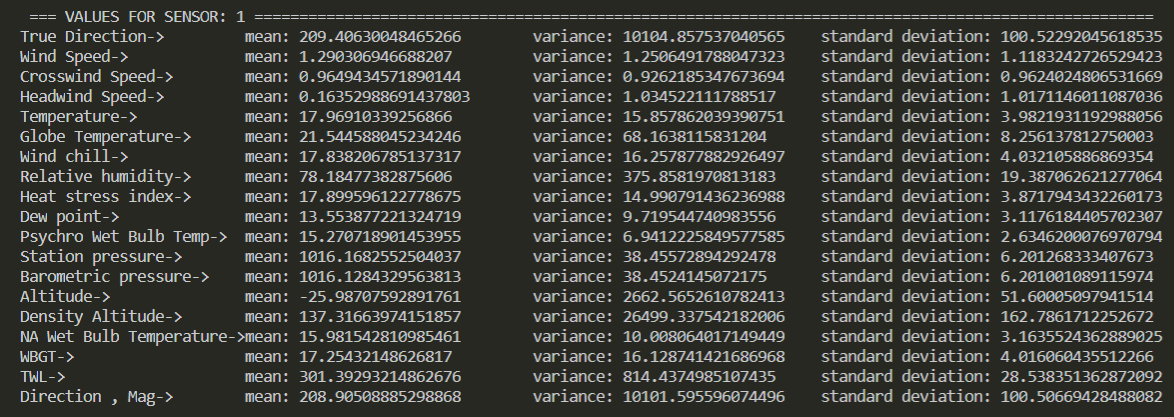
\includegraphics[width=\textwidth]{images/sensor_1.PNG}
            \caption{Sensor A}
            \caption{Statistical indexes}
            
        \end{figure}

        \begin{figure}[H]
            \centering
            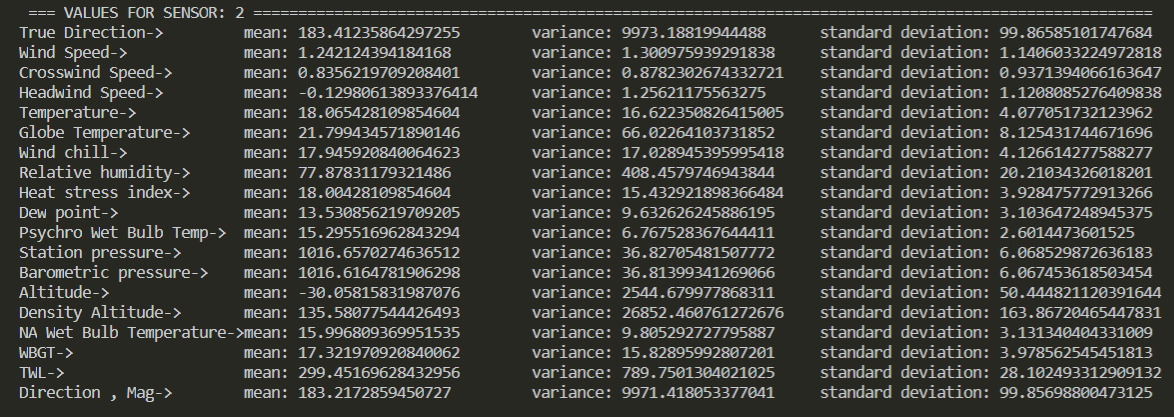
\includegraphics[width=\textwidth]{images/sensor_2.PNG}
            \caption{Sensor B}
            \caption{Statistical indexes}
            
        \end{figure}

        \begin{figure}[H]
            \centering
            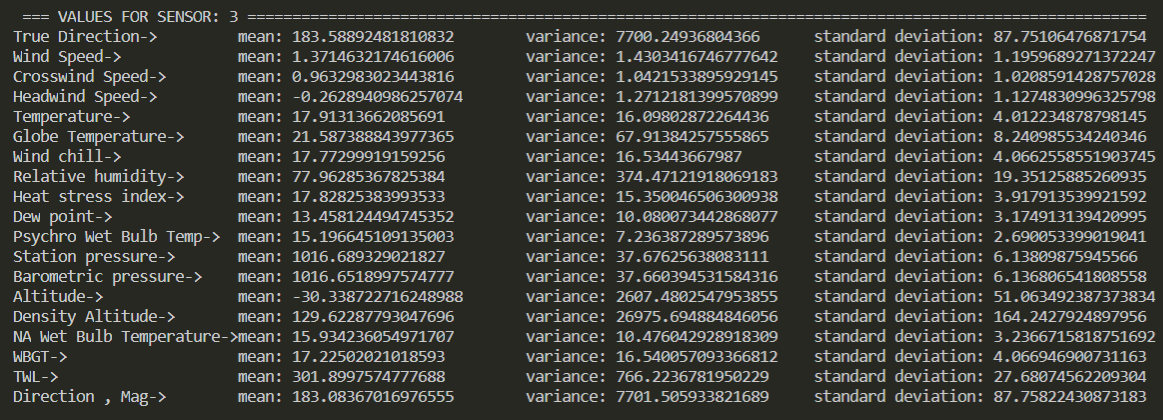
\includegraphics[width=\textwidth]{images/sensor_3.PNG}
            \caption{Sensor C}
            \caption{Statistical indexes}
        
        \end{figure}

        \begin{figure}[H]
            \centering
            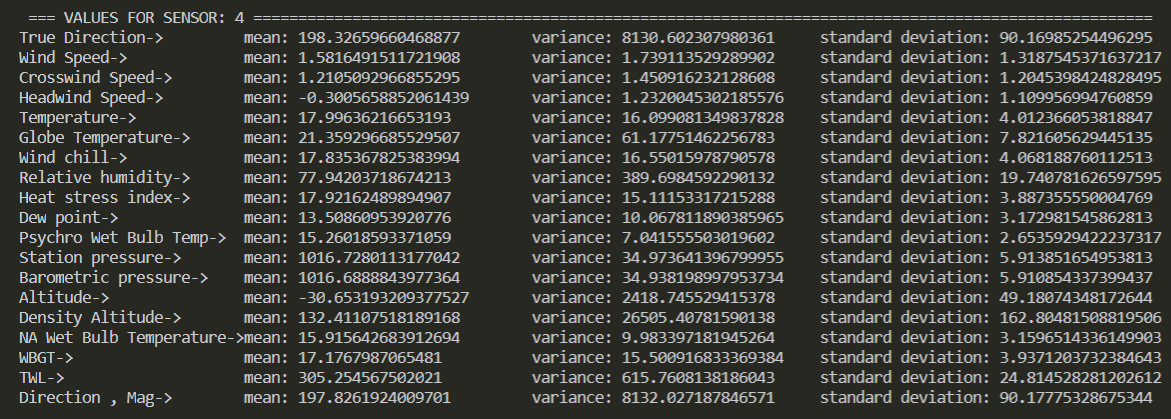
\includegraphics[width=\textwidth]{images/sensor_4.PNG}
            \caption{Sensor D}
            \caption{Statistical indexes}
            
        \end{figure}

        \begin{figure}[H]
            \centering
            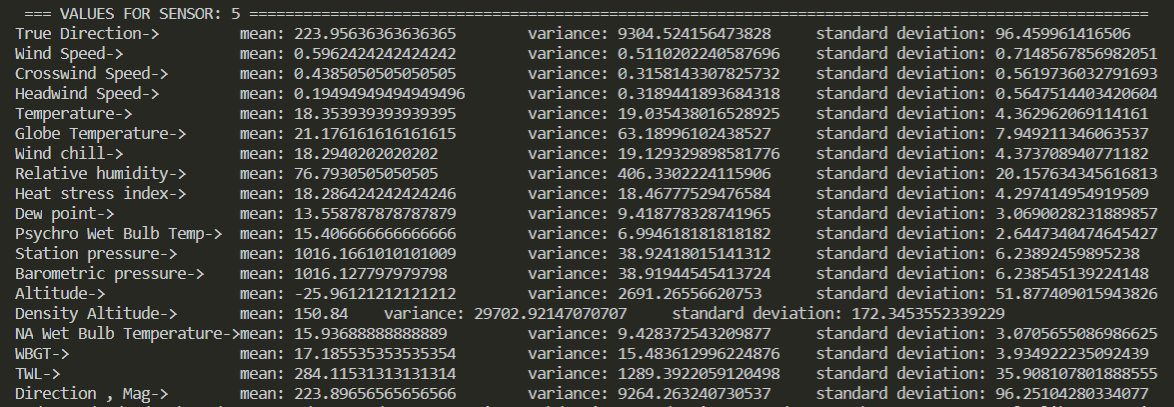
\includegraphics[width=\textwidth]{images/sensor_5.PNG}
            \caption{Sensor E}
            \caption{Statistical indexes}
            
        \end{figure}


    \subsection{Q.2: Create 1 plot that contains histograms for the 5 sensors Temperature values. Compare histograms with 5 and 50 bins, why is the number of bins important?}
    
        Once the required histograms created, the results regarding the importance of bins are the following: 
        \begin{itemize}
            \item The wider the range we used, the fewer columns we had
            \item When bins = 5 we hide important details about distribution while bins = 50 cause a lot of noise and important information about the distribution as well.
            \item Using higher number of bins gives the viewer the ability to distinguish global or local maximums that helps to understand the data’s’ fluctuation.
            \item It is important to use a logical number of bins (depending on the specifications of each project) so on to be easier for the viewer to interpret the data. 
            \item Using too narrow bins results to lots of spikes just by coincidence.
        \end{itemize}

        In general, if we have a small amount of data it is preferable to use wider bins to eliminate noise, otherwise, narrower because the histogram will not be that noisy.

        \begin{figure}[H]
        \centering
            \begin{subfigure}[b]{0.4\linewidth}
              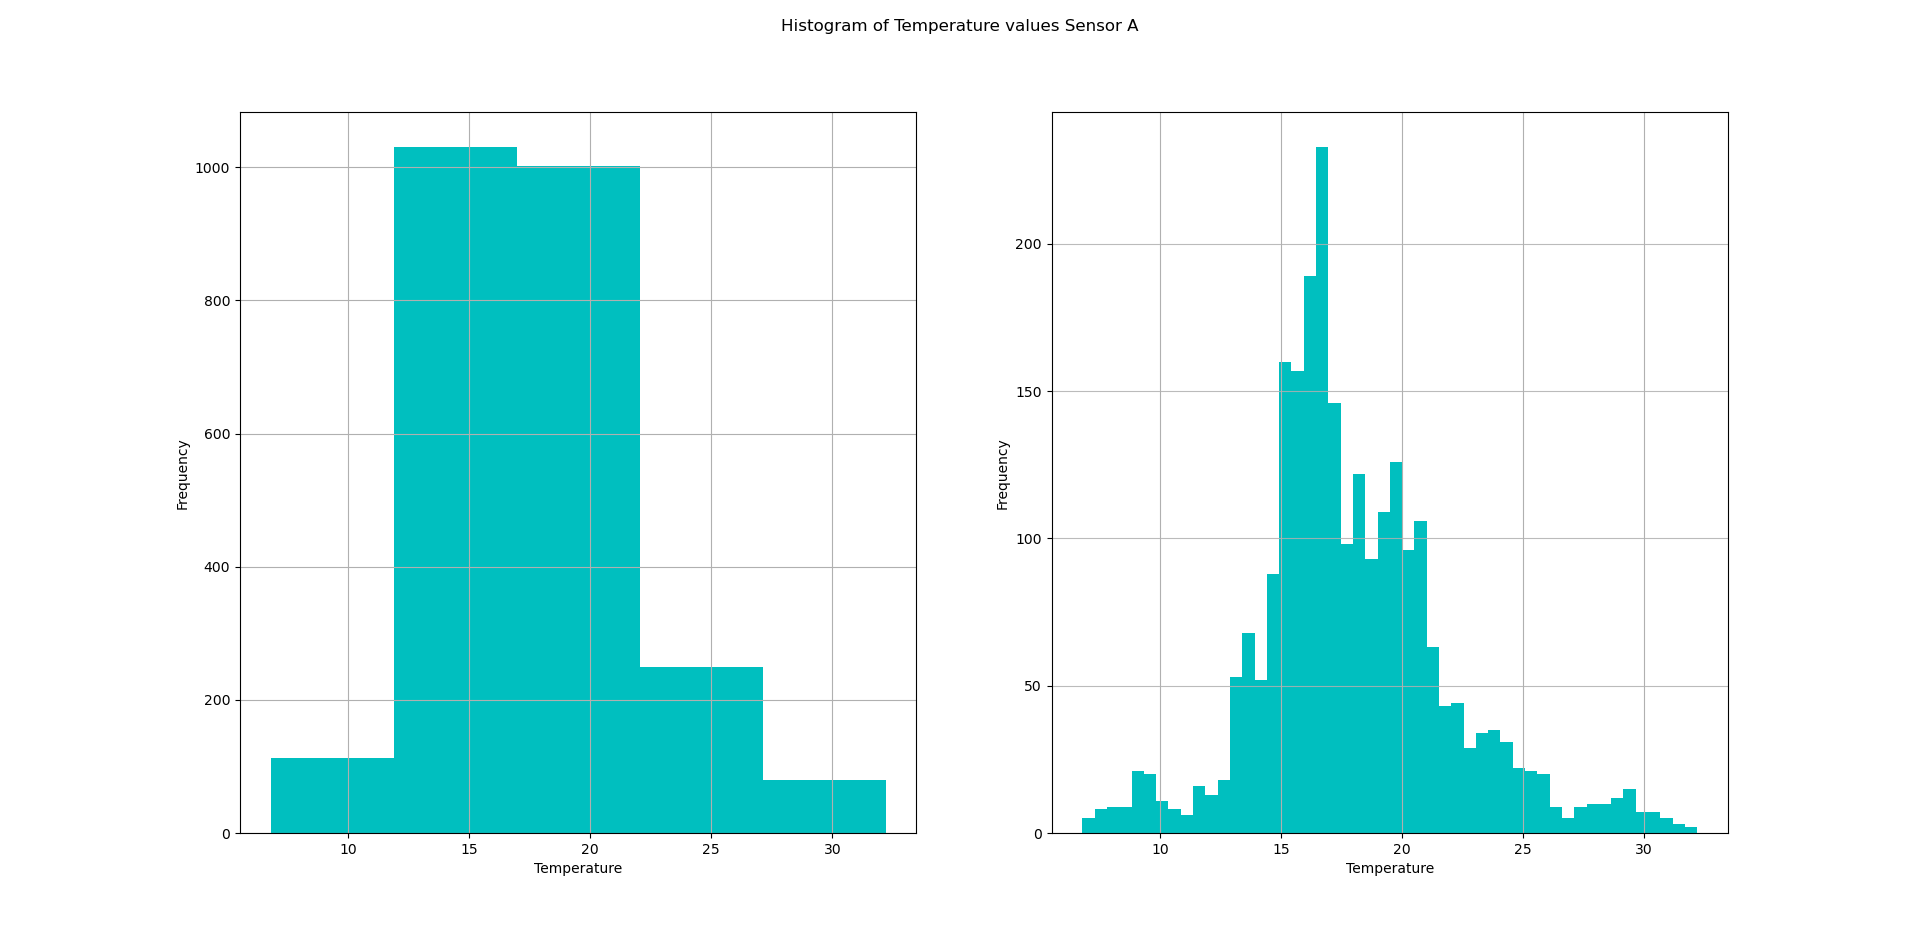
\includegraphics[width=\linewidth]{images/Histogram_of_Temperature_values_Sensor_A.png}
              \caption{Sensor A}
            \end{subfigure}
            \begin{subfigure}[b]{0.4\linewidth}
              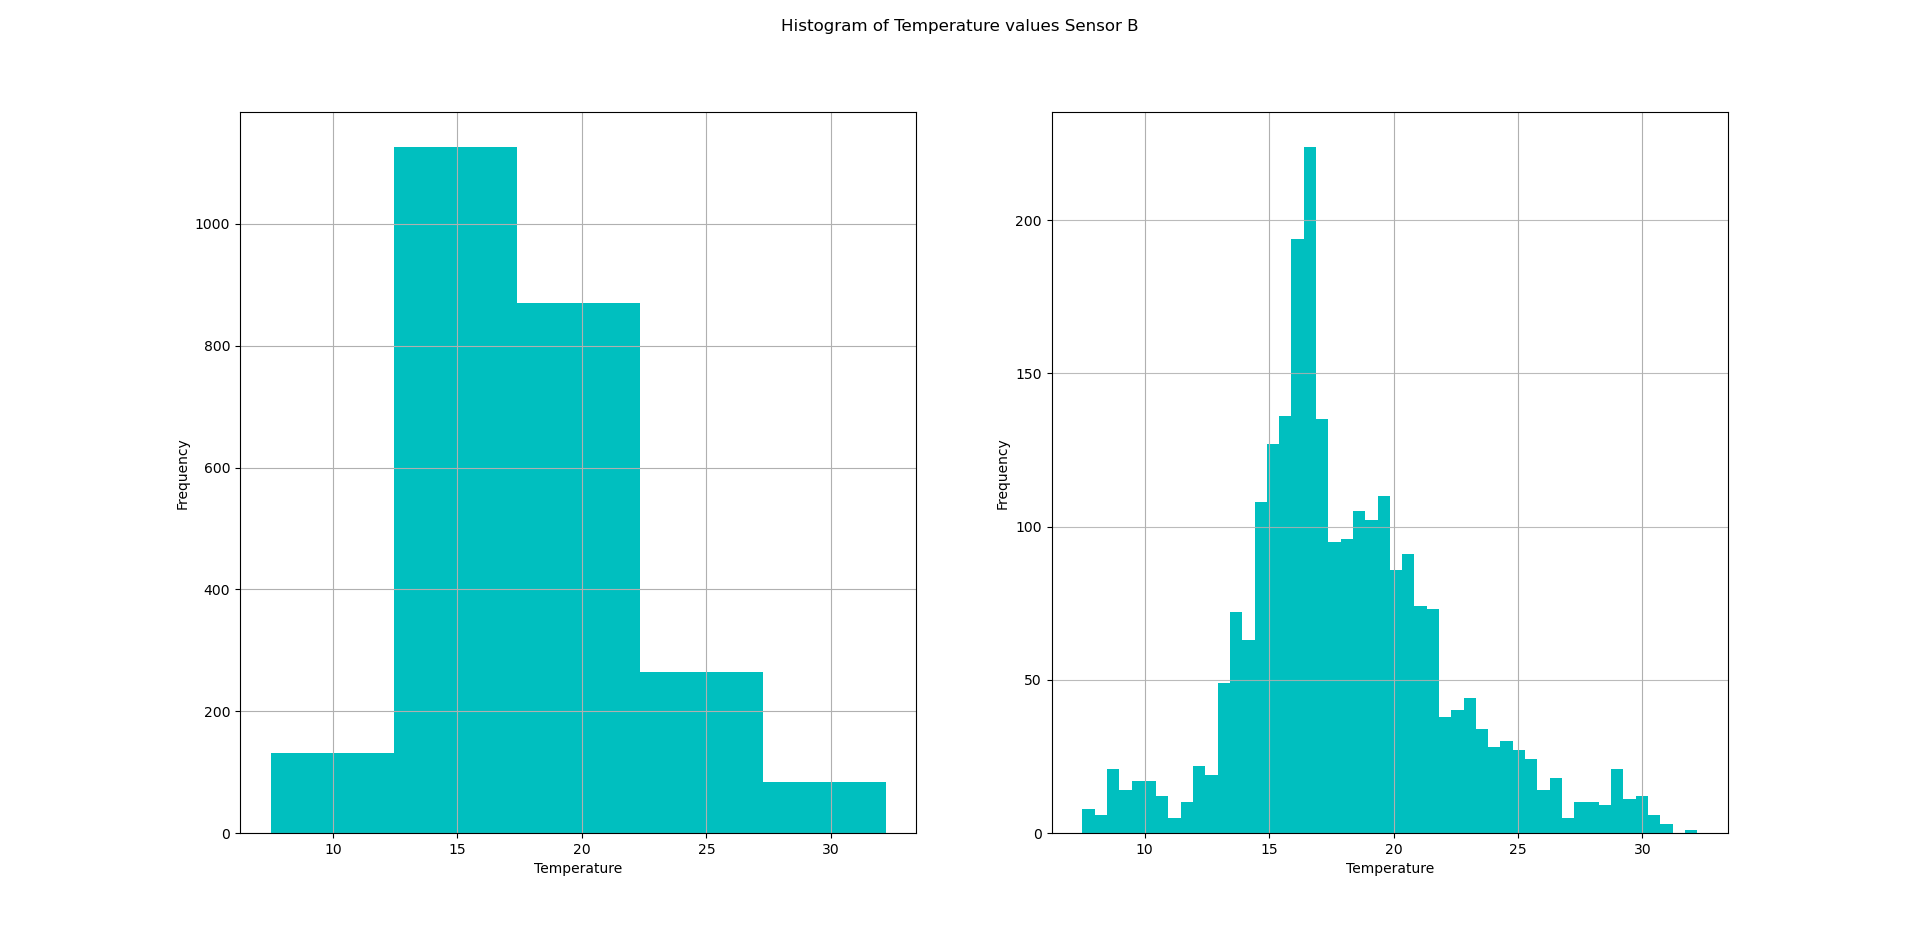
\includegraphics[width=\linewidth]{images/Histogram_of_Temperature_values_Sensor_B.png}
              \caption{Sensor B}
            \end{subfigure}
            \caption{Temperature histograms: bins = 5, bins = 50}
            \label{fig:Histogram}
        \end{figure} 
        
        \begin{figure}[H]
            \centering
            \begin{subfigure}[b]{0.4\linewidth}
              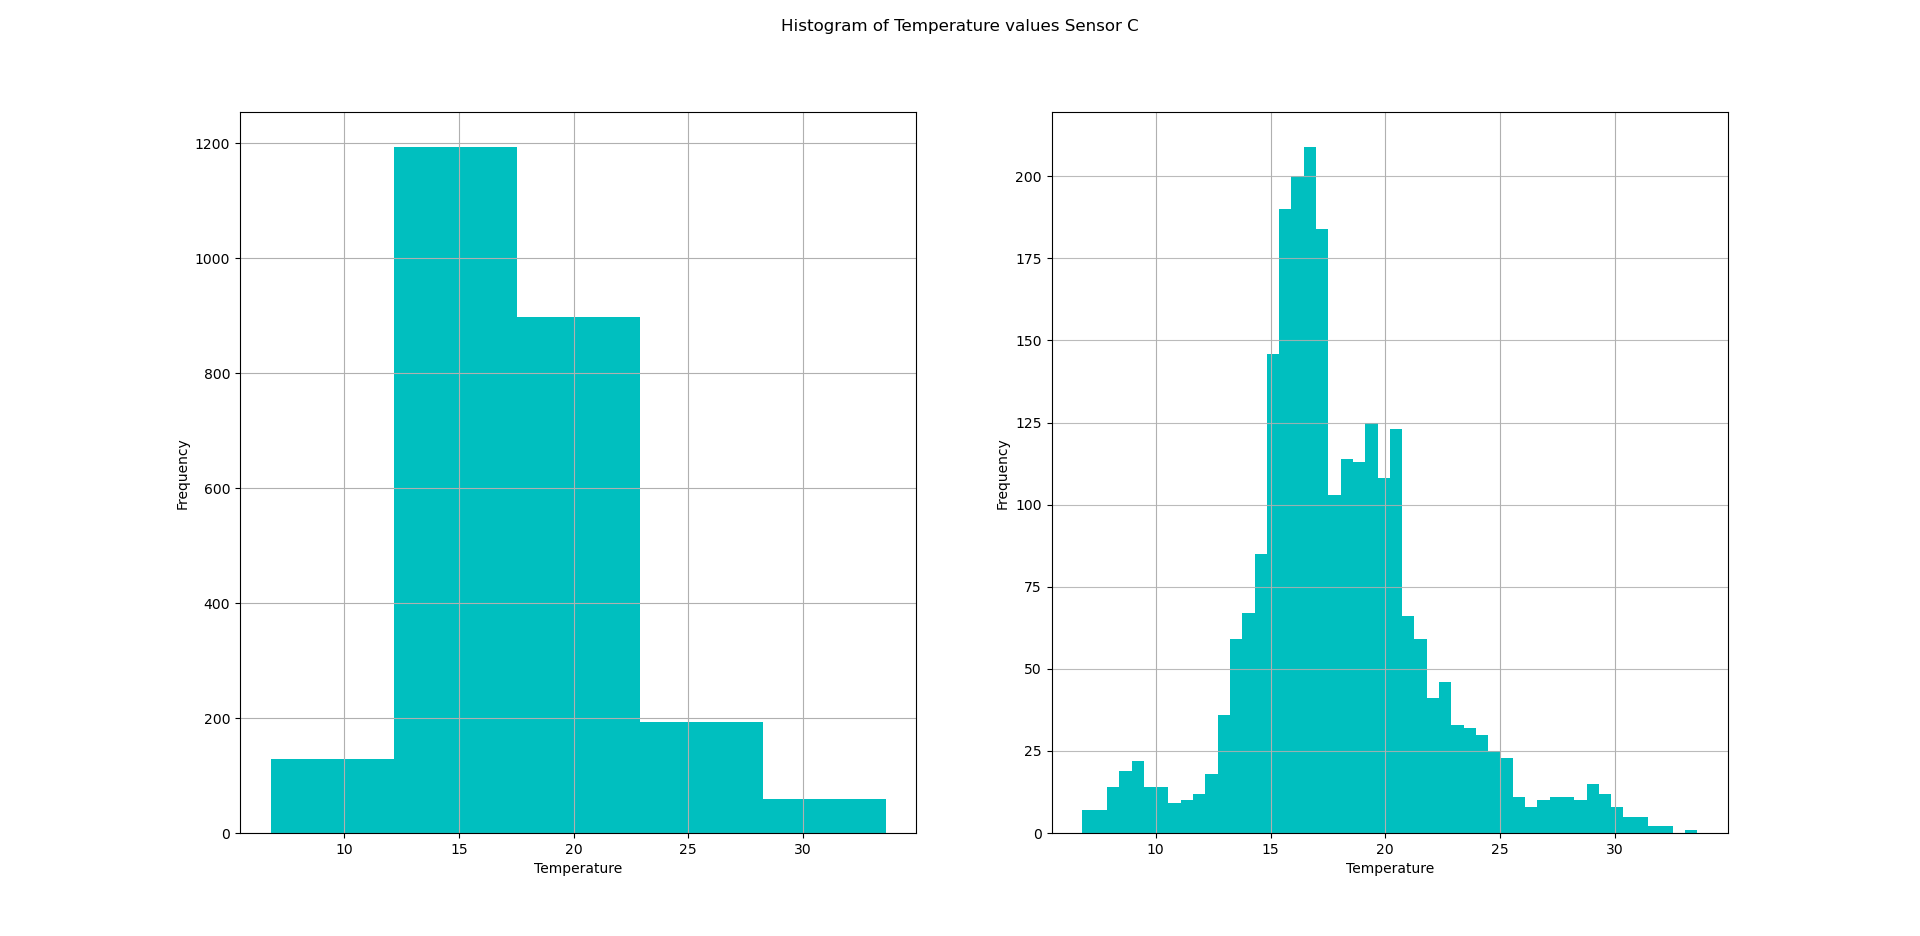
\includegraphics[width=\linewidth]{images/Histogram_of_Temperature_values_Sensor_C.png}
              \caption{Sensor C.}
            \end{subfigure}
            \begin{subfigure}[b]{0.4\linewidth}
              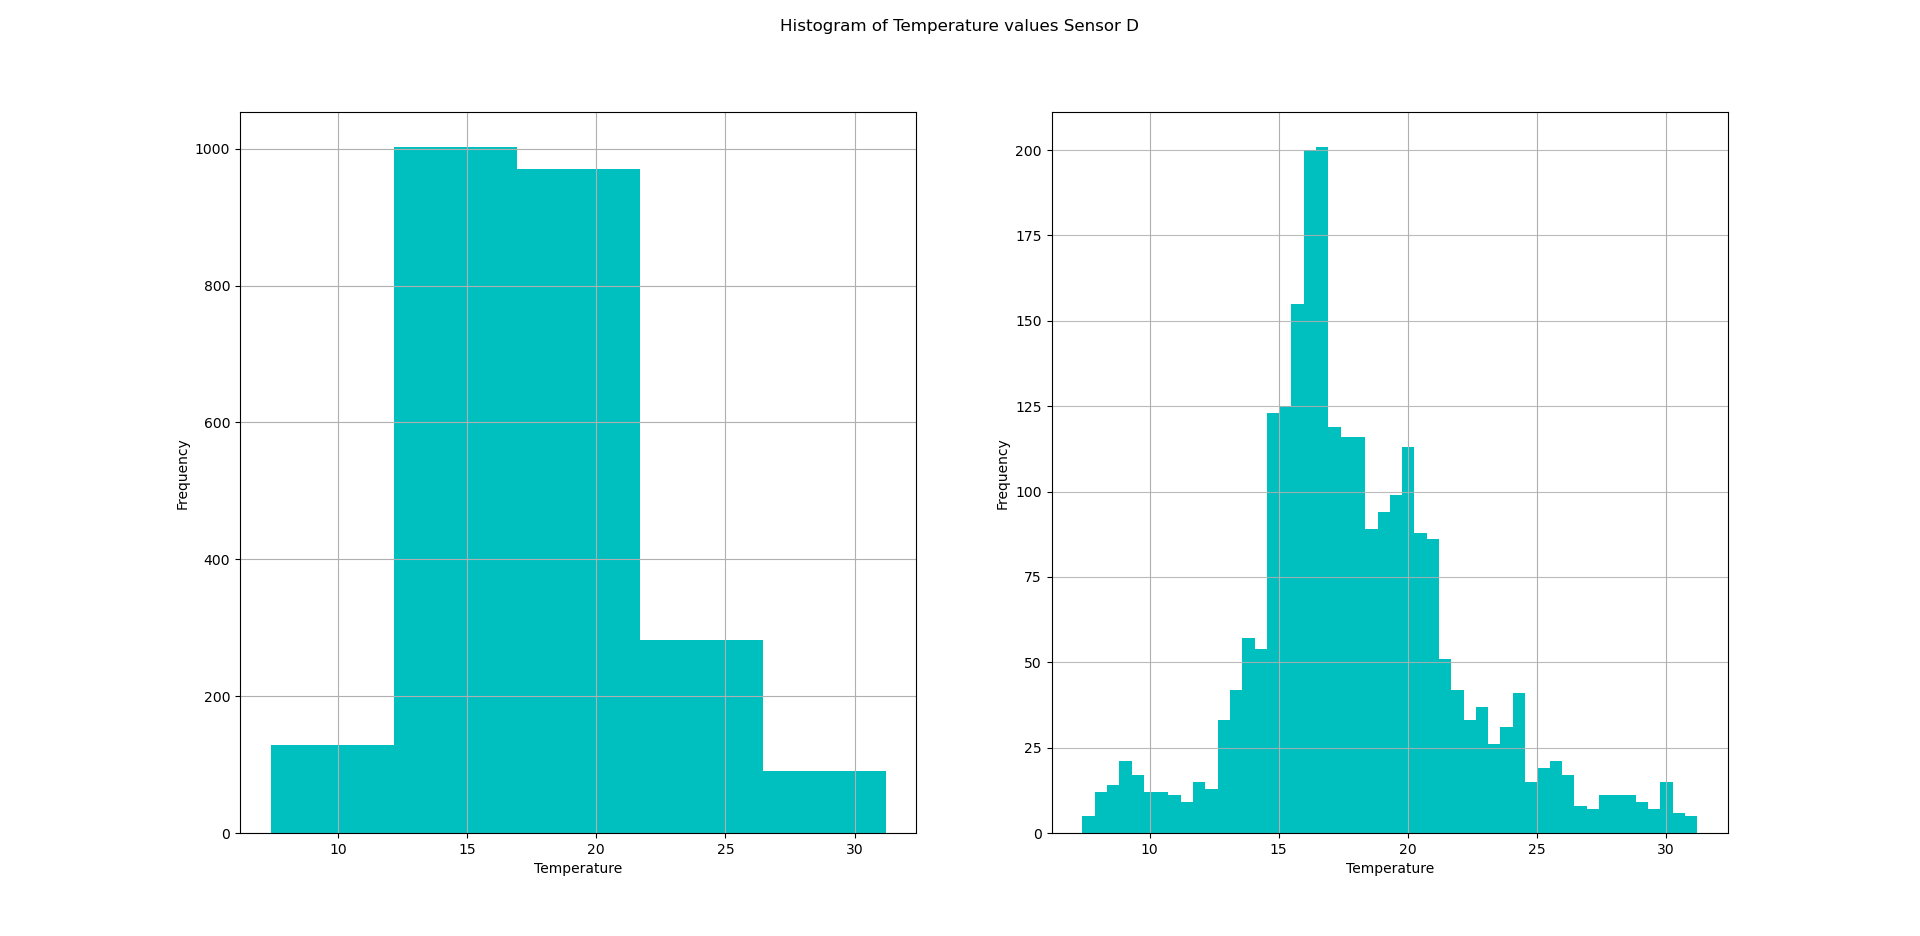
\includegraphics[width=\linewidth]{images/Histogram_of_Temperature_values_Sensor_D.png}
              \caption{Sensor D}
            \end{subfigure}
            \caption{Temperature histograms: bins = 5, bins = 50}
            \label{fig:Histogram}
        \end{figure} 


        \begin{figure}[H]
        \centering
            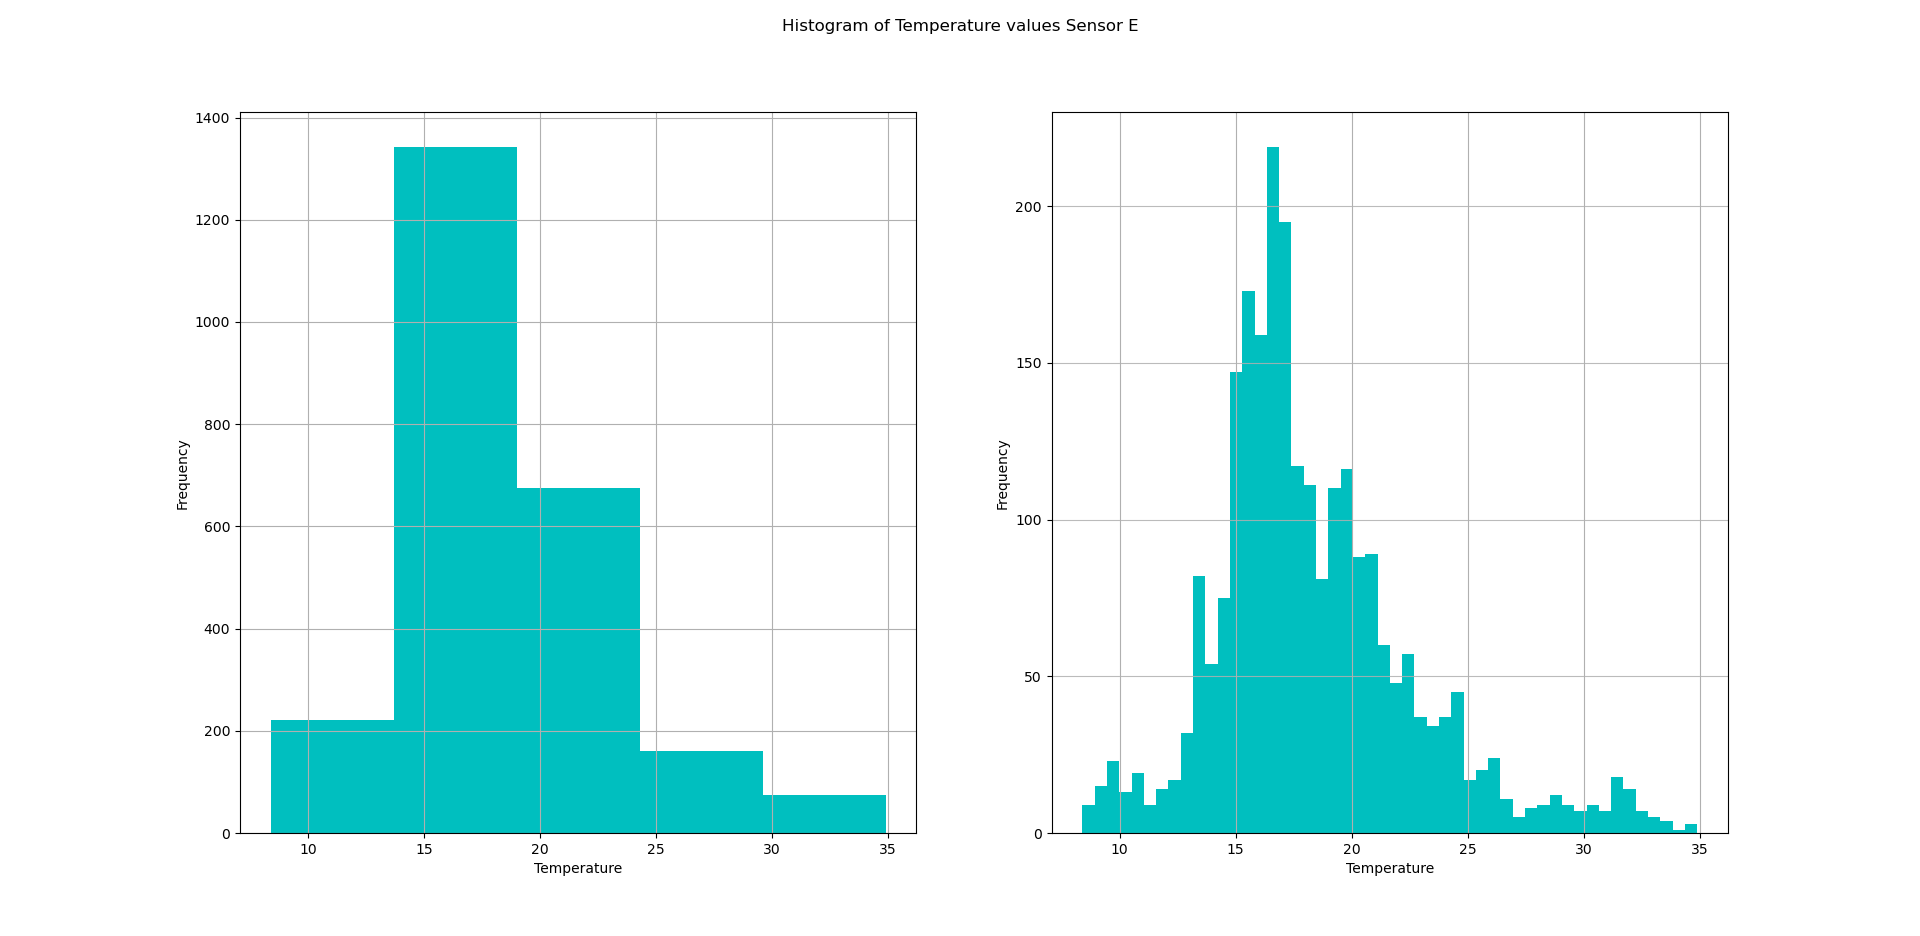
\includegraphics[width=0.5\textwidth]{images/Histogram_of_Temperature_values_Sensor_E.png}
            \caption{Sensor E}
            \caption{Tempreture histogram with bins=5 , bins=50}
            \label{fig:Histogram}
        \end{figure}
    
    \subsection{Q.3: Create 1 plot where frequency poligons for the 5 sensors Temperature values overlap in different colors with a legend.}
    
        In question A1:Q3, a frequency polygons plot created for all the sensors, for the “Temperature” variable. The results obtained are as follows:
        
            \begin{figure}[H]
            \centering
                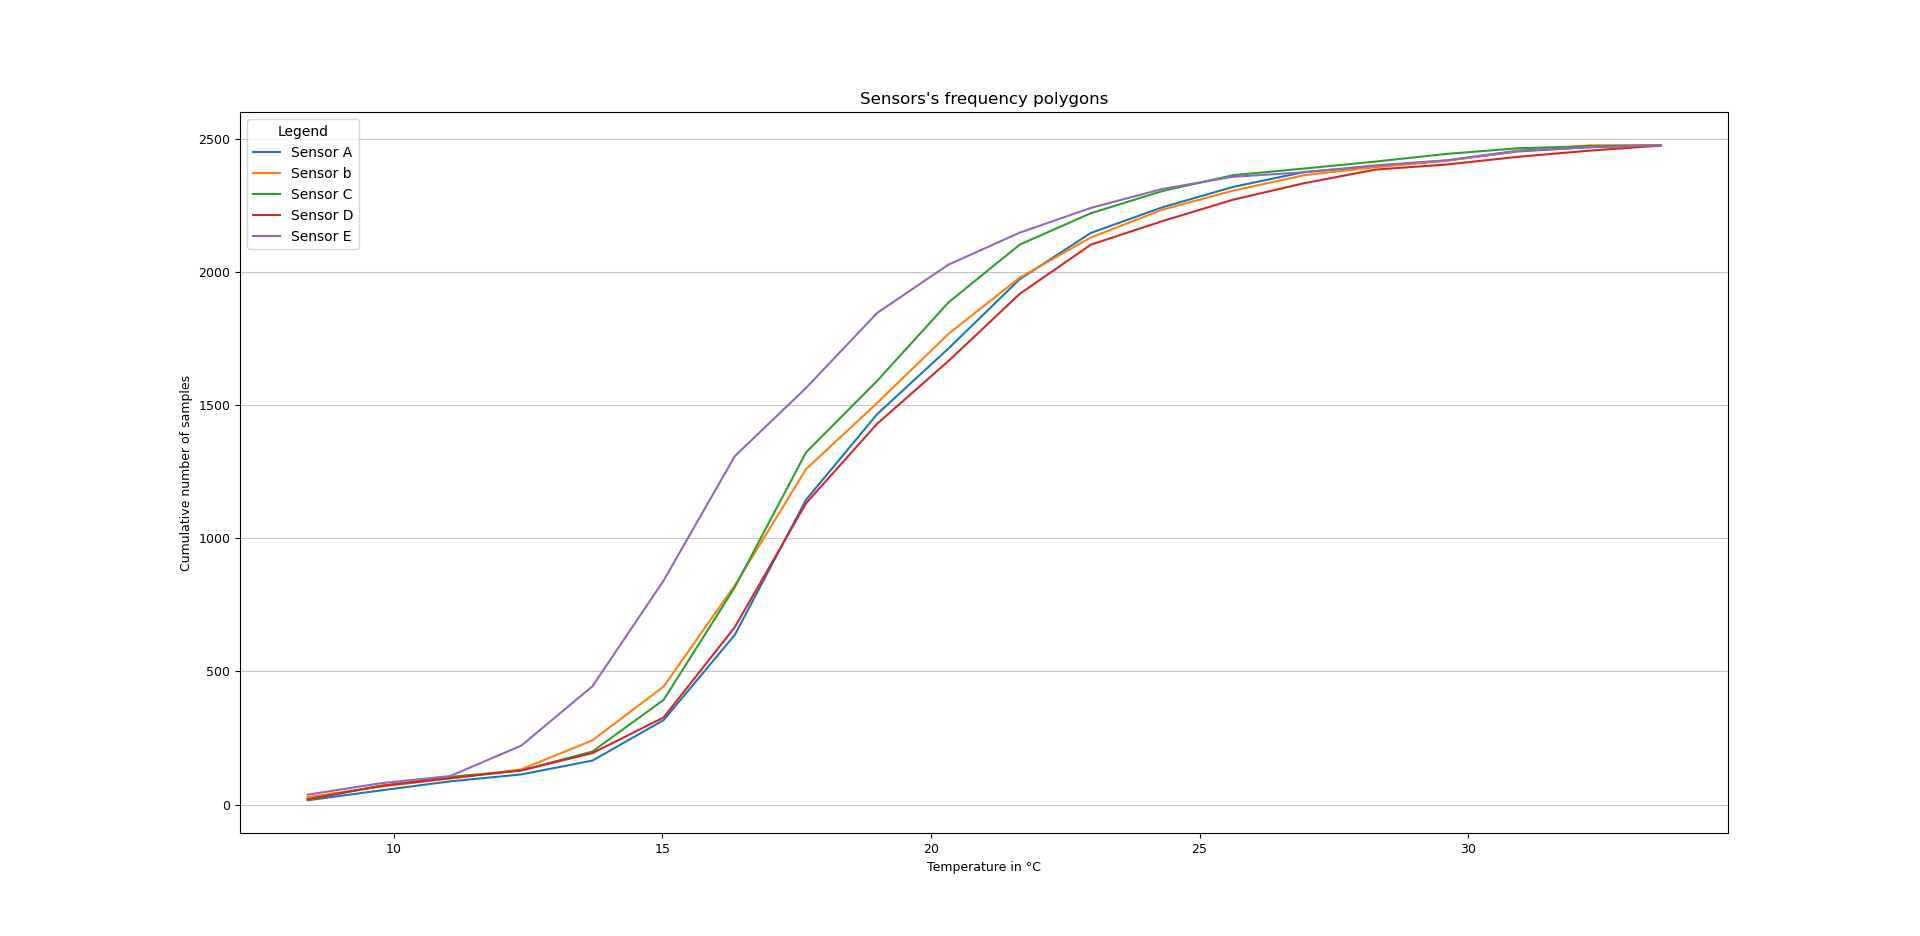
\includegraphics[width=\textwidth]{images/Frequency_polygons.png}
                \caption{Frequenncy polygon plot for Temperature}
                \label{fig:Frequency polygons}
            \end{figure}

        Through the frequency’s polygon plot we can understand the shape of the distribution and they are helpful for comparing the different sets of data. The given plot illustrates information about the frequency of each sensor for the variable of Temperature. It is clear that the majority of sensors follow a same temperature pattern expect from sensor E that seems to have its highest percentage of (temperature) values between 15°C and 24 °C. 

   
    \subsection{Q.4: Generate 3 plots that include the 5 sensors boxplot for: Wind Speed, Wind Direction and Temperature.}
     Another way to represent visually our data is boxplots. In this case, apart from comparing distributions we receive also important information for the outliers. Through boxplots and its’ elements (minimum, maximum, sample median, and first and third quartiles) we can understand the behavior of a distribution. For example through Winds’ Direction boxplot and its y-label values we can estimate winds’ cardinal direction an important information that will helps us, as we will see below, to discern the possible positions of the sensors. Moreover, the former boxplot depicts information about the skewness of the distribution. Comparing the mean with the median helps us to clarify if the distribution has a positive or negative skew (mean>median --> positive skew).

        \begin{figure}[H]
            \centering
            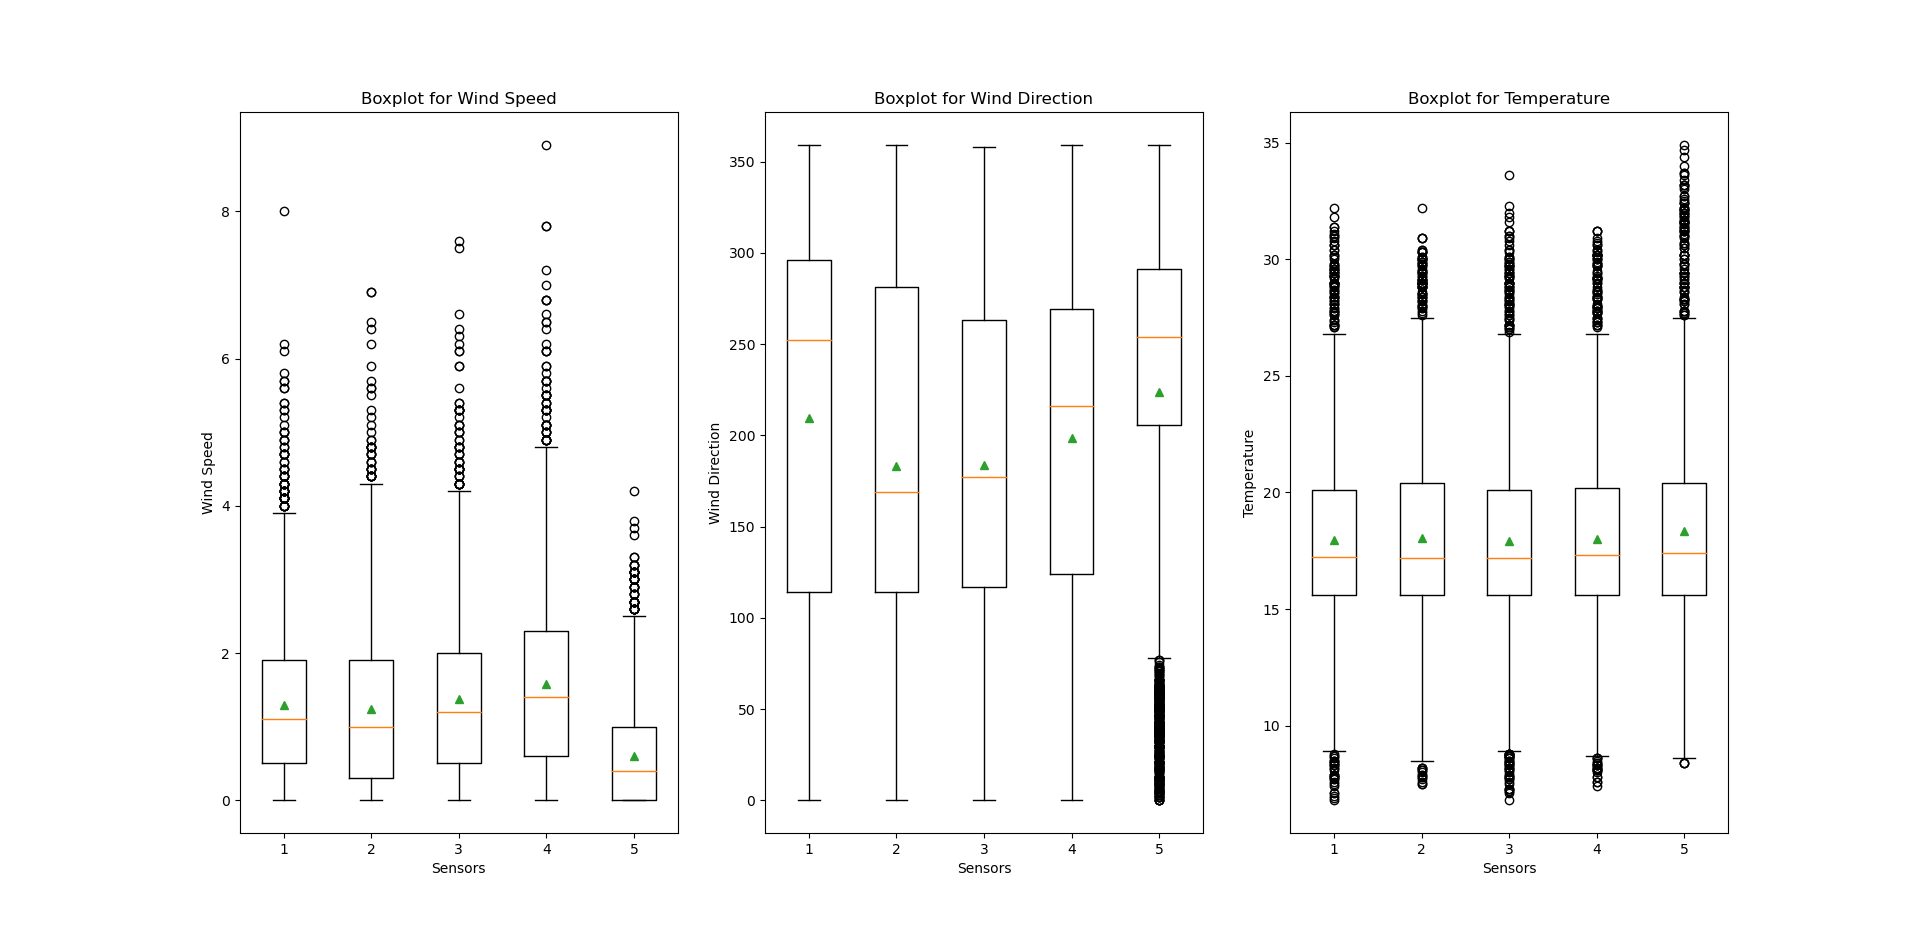
\includegraphics[width=\textwidth]{images/Boxplots_for_the_three_variables.png}
            \caption{Wind Speed, Wind Direction and Temperature boxplots}
            \label{fig:Boxplot}
        \end{figure}
        
        
\section{Part II}

        \subsection{Q.1: Plot PMF, PDF and CDF for the 5 sensors Temperature values in independent plots (or subplots). Describe the behaviour of the distributions, are they all similar? what about their tails?}
        
            Comparing the PMF, PDF and CDF temperature graphs for each sensor we see that they show significant similarities and follow similar patterns. 
            Probability Mass Distribution, in general, gives the probability that a discrete random variable is exactly equal to some value. Probability Density Function of a continuous random variable, is a function whose value at any given sample (or point) in the sample space (the set of possible values taken by the random variable) can be interpreted as providing a relative likelihood that the value of the random variable would equal that sample. Regarding PMF and PDF we see that they are quite similar. They are higher in the middle compared to its two tails. Their tail in the positive direction extends further than the tail in the negative one (right-skewed). Moreover they both range from almost 4°C to 35°C and reach a top of 0.024 and 0.016, PMF and PDF respectively.
            As far as CDF is concerned, is the probability that the variable takes a value less than or equal to x. In this plot is observed that there are no significant changes in CDFs form whilst all sensors appear to follow a similar pattern of distribution on their temperatures. 

            \begin{figure}[H]
            \centering
                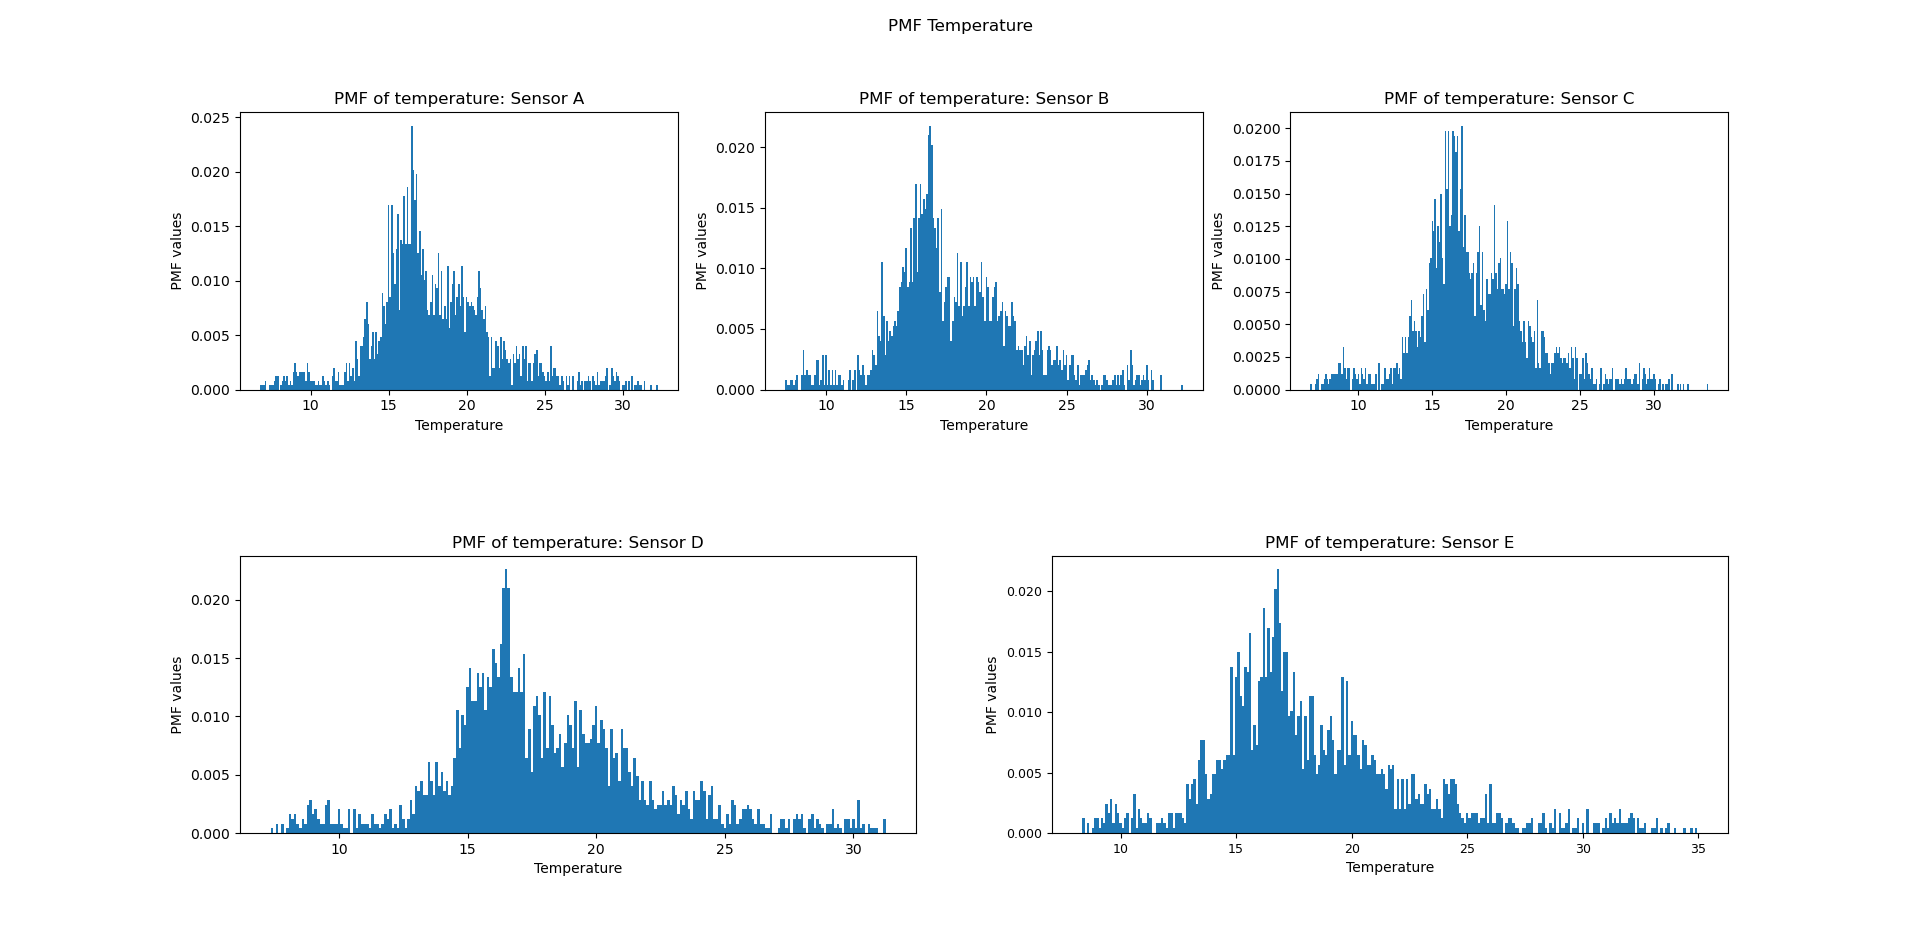
\includegraphics[width=\textwidth]{images/PMF_Temperature_5_sensors.png}
                \caption{Probability Mass Function for Temperature}
                \label{fig:Sensors's PMF}
            \end{figure}

            \begin{figure}[H]
            \centering
                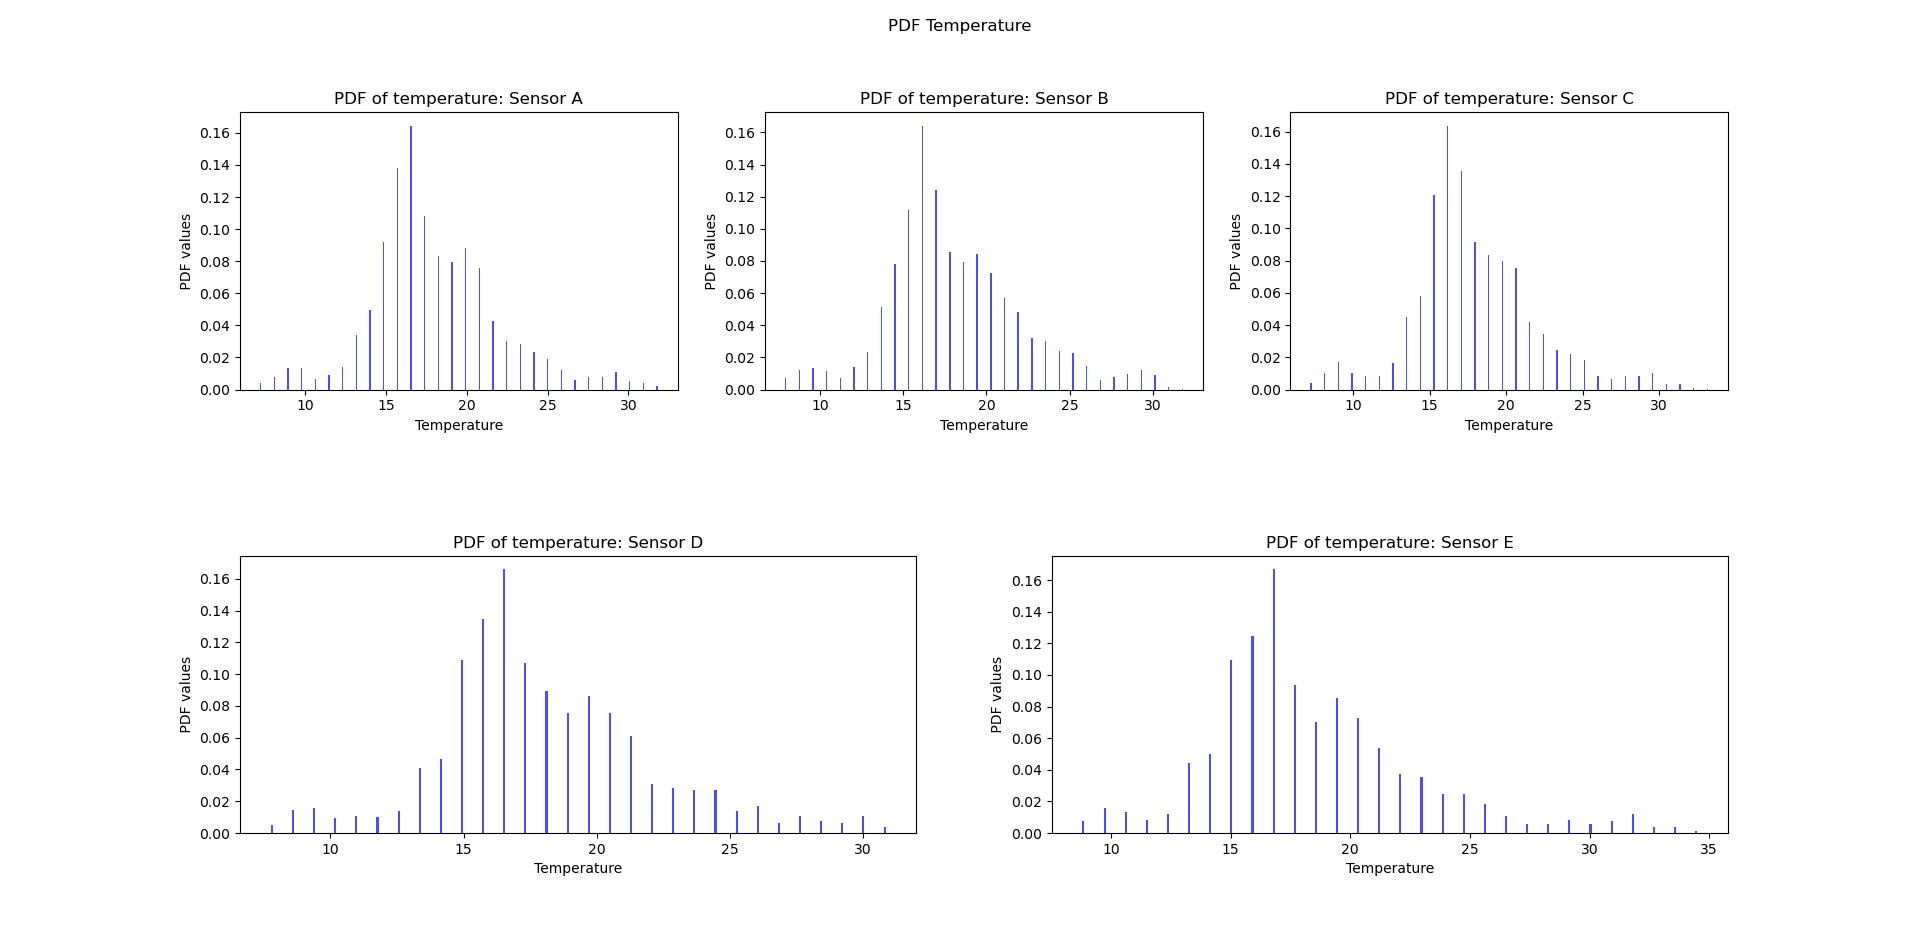
\includegraphics[width=\textwidth]{images/PDF_Temperature_5_sensors.png}
                \caption{Probability Density Function}
                \label{fig:Sensors's PDF}
            \end{figure}

            \begin{figure}[H]
            \centering
                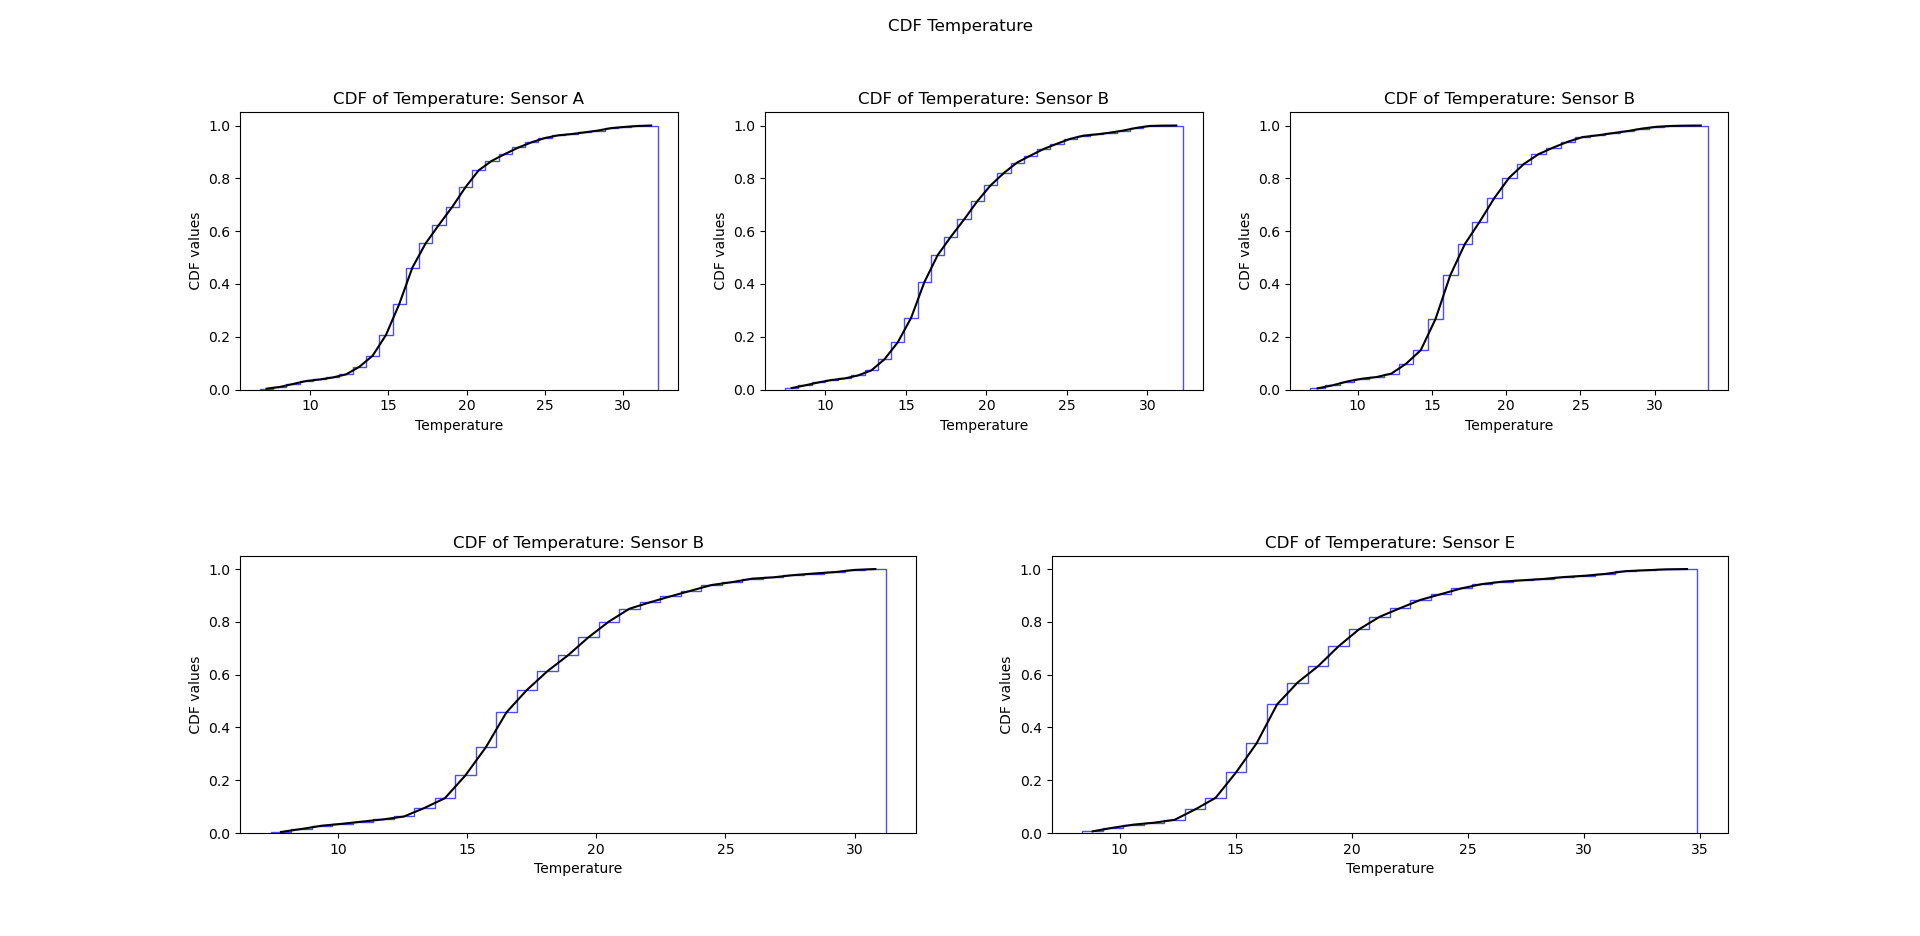
\includegraphics[width=\textwidth]{images/CDF_Temperature_5_sensors.png}
                \caption{Cumulative Density Function}
                \label{fig:Sensor's CDF}
            \end{figure}

        \subsection{Q.2:For the Wind Speed values, plot the pdf and the kernel density estimation. Comment the differences.}
        
            Analyzing Kernel’s Density Estimation plot we noticed a smoother presentation of the data, a fact that results from KDEs way of working (plotting out the data and beginning to create a curve of the distribution). Since KDE is an algorithm that estimates a PDF (based on a sample) the main difference between them is that the former one gives a general visualization of the data and this may cause the lost of some extreme values. The majority of sensors (A, B, C, D) shows a range of wind speed between 0 and 8 [m/s], apart from sensor E, who did not surpass the speed of 3 [m/s]. Regarding the wind speed values we can estimate that sensor E is located at a point which is not so affected from the wind. 
            \begin{figure}[H]
            \centering
                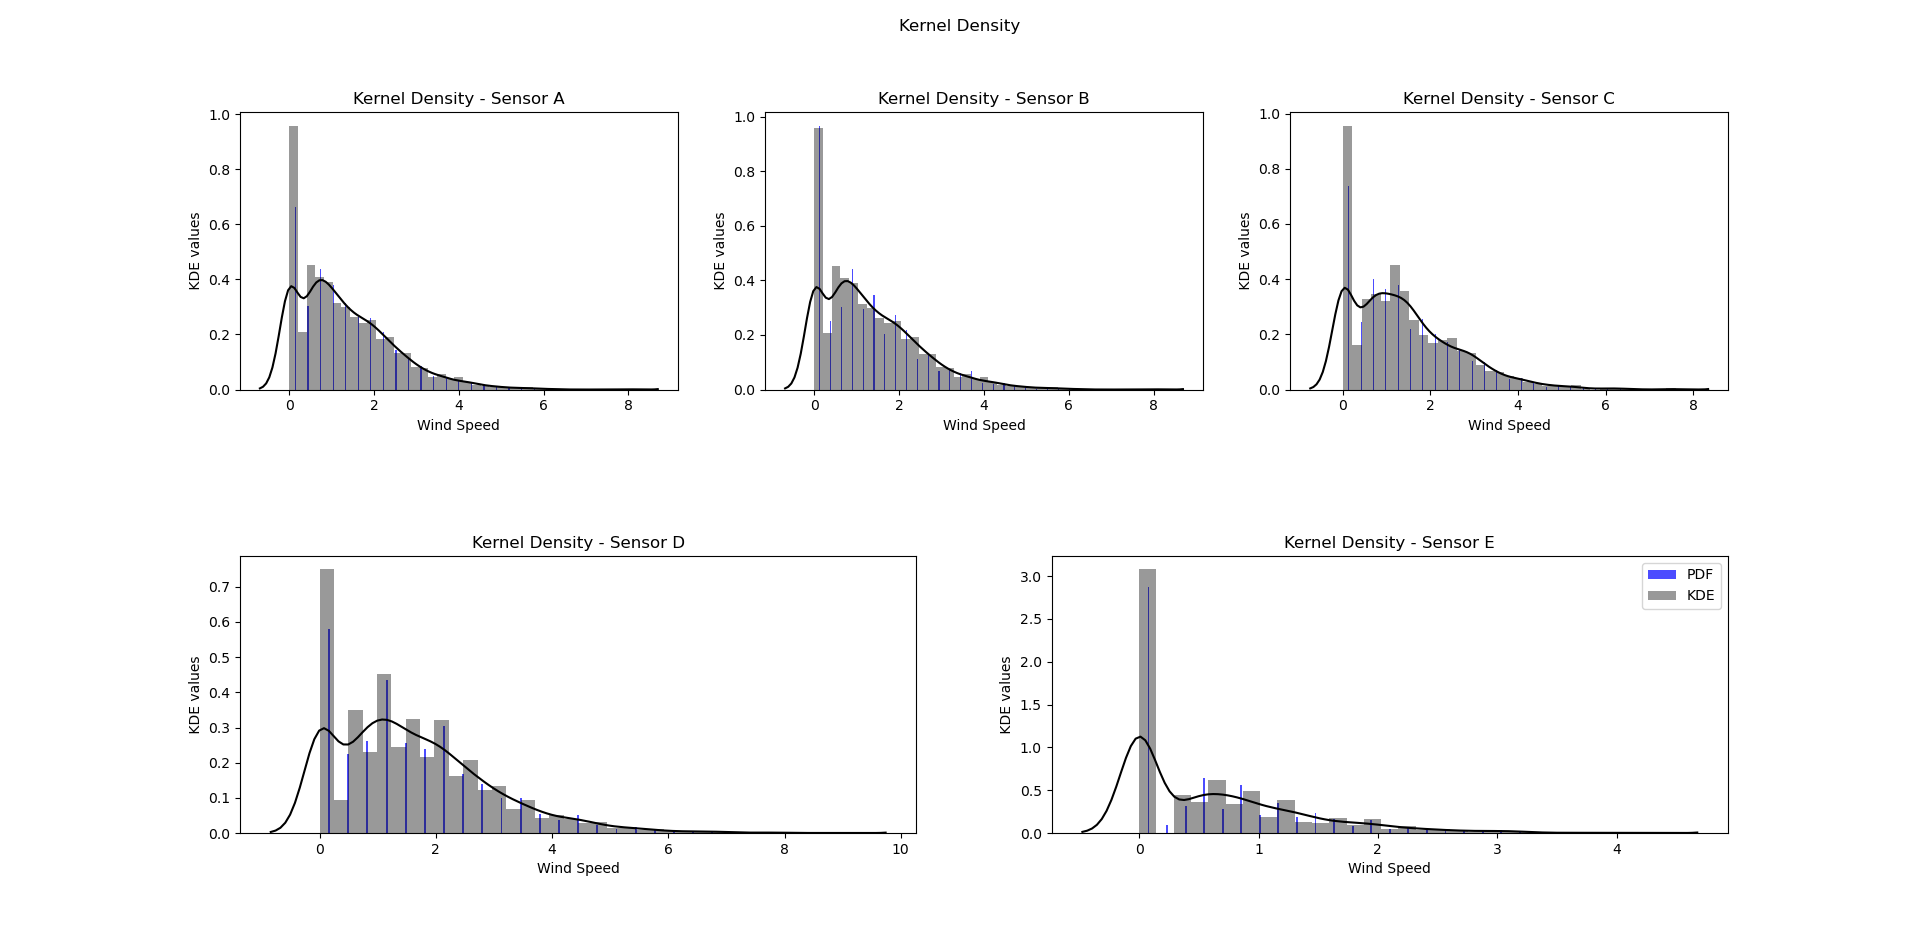
\includegraphics[width=\textwidth]{images/Kernel_Density.png}
                \caption{Kernel Density for Wind Speed}
                \label{fig:Kernel Density}
            \end{figure}

\section*{Part III}

        \subsection{Q.1:Pearson's - Spearman's correlations}
        Question A1:Compute the correlations between all the sensors for the variables: Temperature, Wet Bulb Globe Temperature (WBGT), Crosswind Speed. Perform correlation between sensors with the same variable, not between two different variables; for example, correlate Temperature time series between sensor A and B. Use Pearson’s and Spearmann’s rank coefficients. Make a scatter plot with both coefficients with the 3 variables.
        Question A1.1: What can you say about the sensors’ correlations?
        Question A1.2: If we told you that that the sensors are located as follows, hypothesize which location would you assign to each sensor and reason your hypothesis using the correlations.

            In order to quantify the strength of the relationship between the requested variables (Temperature, Wet Bulb Globe, Crosswind) for all the sensors, Pearson’s and Spearman’s rank coefficients computed. 
            With Pearson’s correlation each value transformed to a standard score, which is the number of standard deviations from the mean since with Spearman’s correlation each value transformed to its rank, which is its index in the sorted list of values. 
            Comparing the outcomes of both rank coefficients for all sensors we observed that the combinations of the sensors A, B, C, D with E show less correlation, with AE and BE having the lowest one, concerning the variables of Temperature and Crosswind respectively. For the tested variables sensors A-C, B-D have the strongest positive connection (about 0.98) which is an indication useful for finding the possible location of the sensors. 
            On Cross Wind Speed scatter plot Spearman’s rank coefficients fluctuated between 0.530 – 0.600 whilst Pearson’s between 0.400-0.560. These values differ significantly compared to the correlation values shown in the Temperature and Wet Bulb Globe scatter plots. However, both values represent also strong correlations and in this case is observed that sensors B-E have the lowest correlations (comparing with the other values).

            \begin{figure}[H]
            \centering
                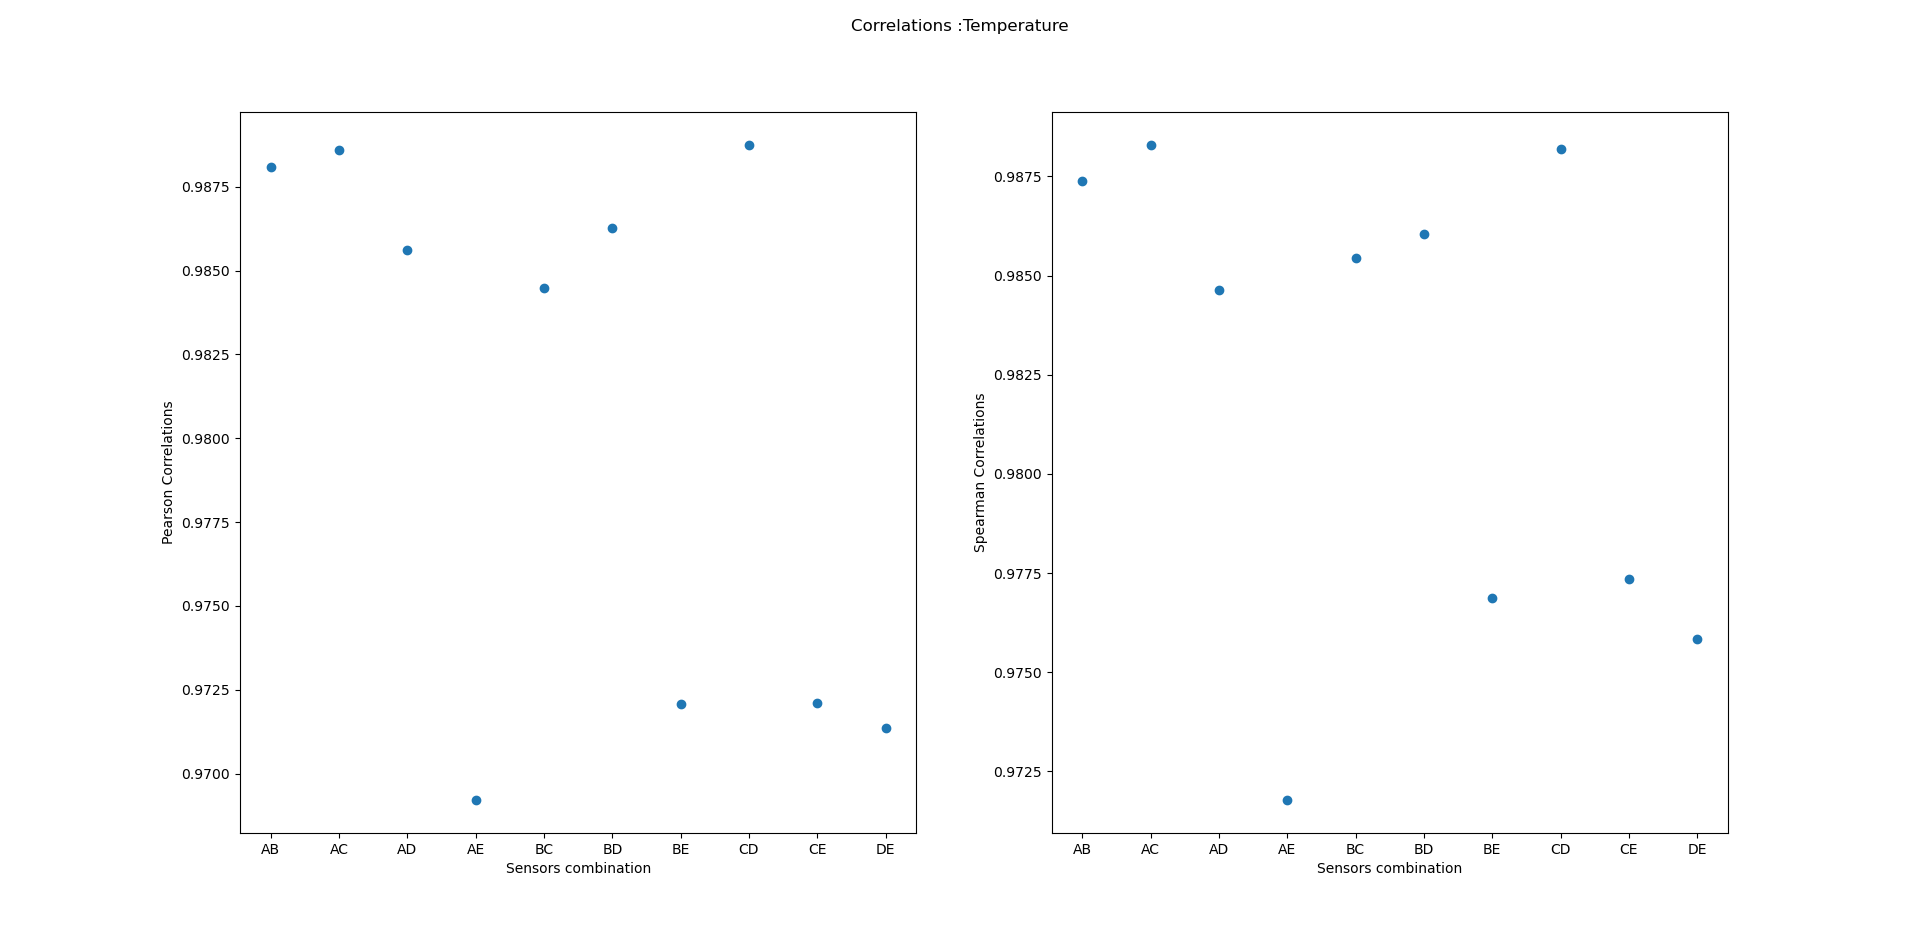
\includegraphics[width=\textwidth]{images/Correlation_Temperature.png}
                \caption{Pearson’s and Spearman’s rank coefficients: Temperature}
                \label{fig:Correlations}
            \end{figure}

            \begin{figure}[H]
            \centering
                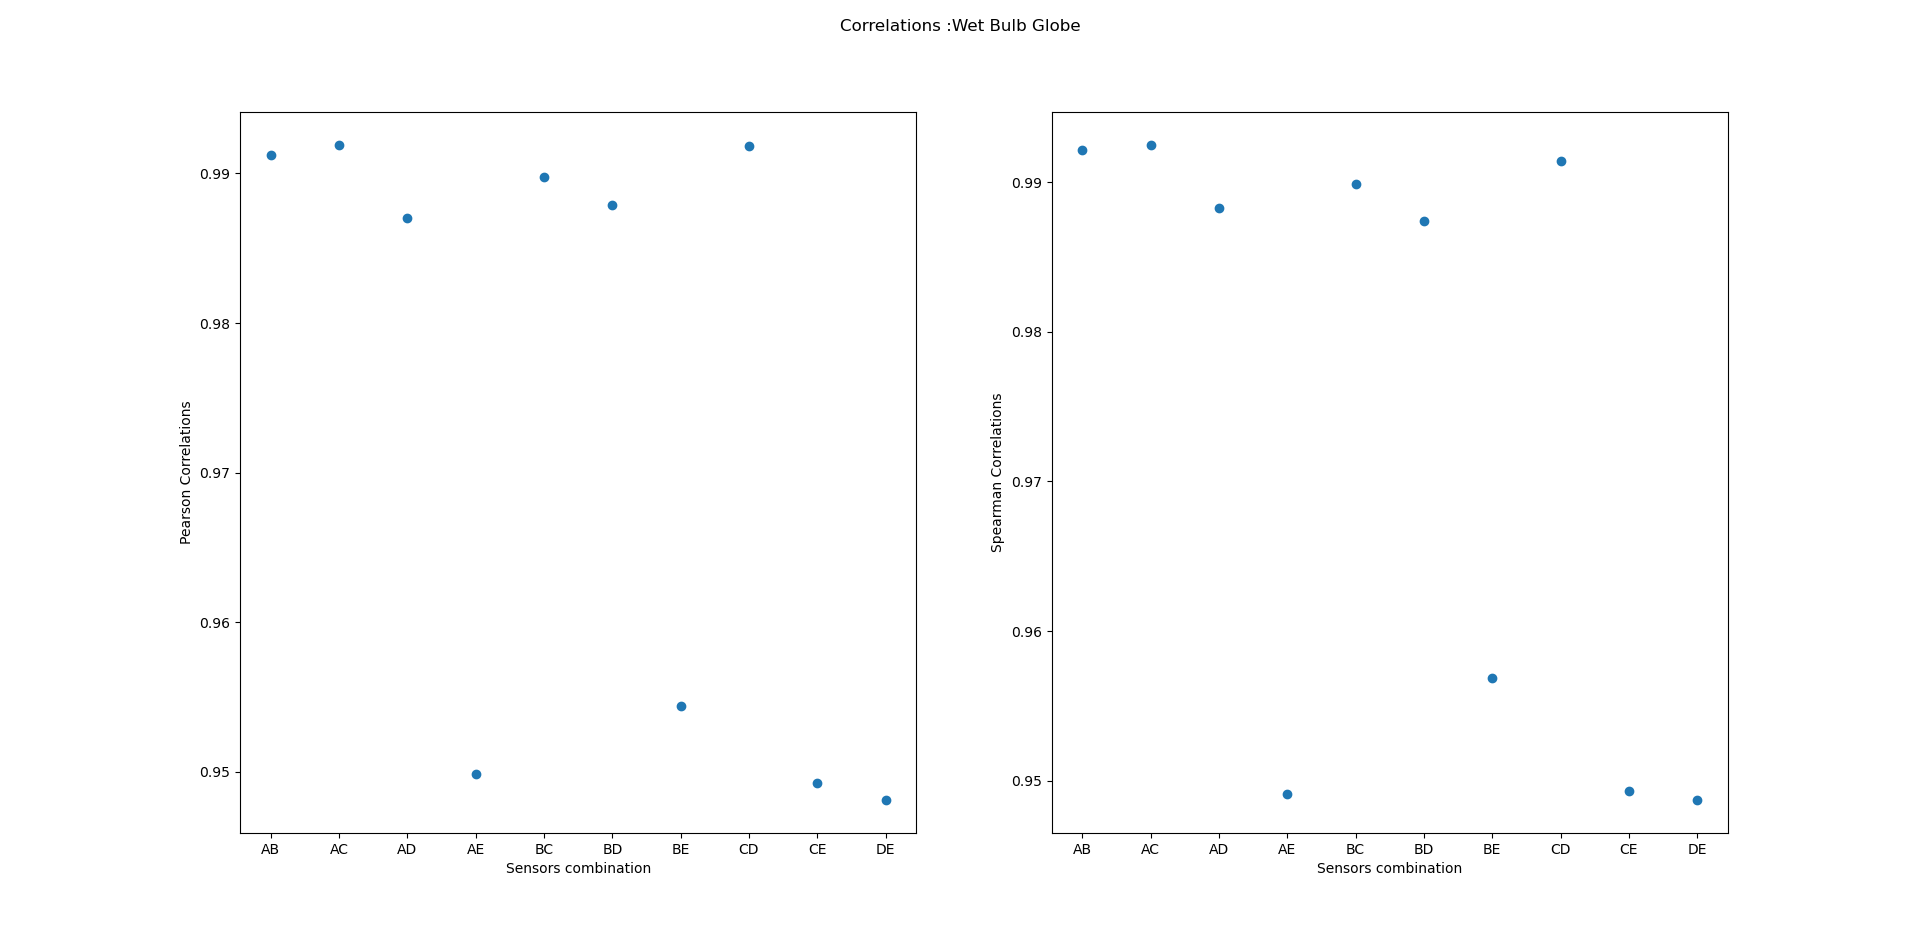
\includegraphics[width=\textwidth]{images/Correlation_Wet_bulb_Globe.png}
                \caption{Pearson’s and Spearman’s rank coefficients: Wet Bulb Globe}
                \label{fig:Correlations}
            \end{figure}

            \begin{figure}[H]
            \centering
                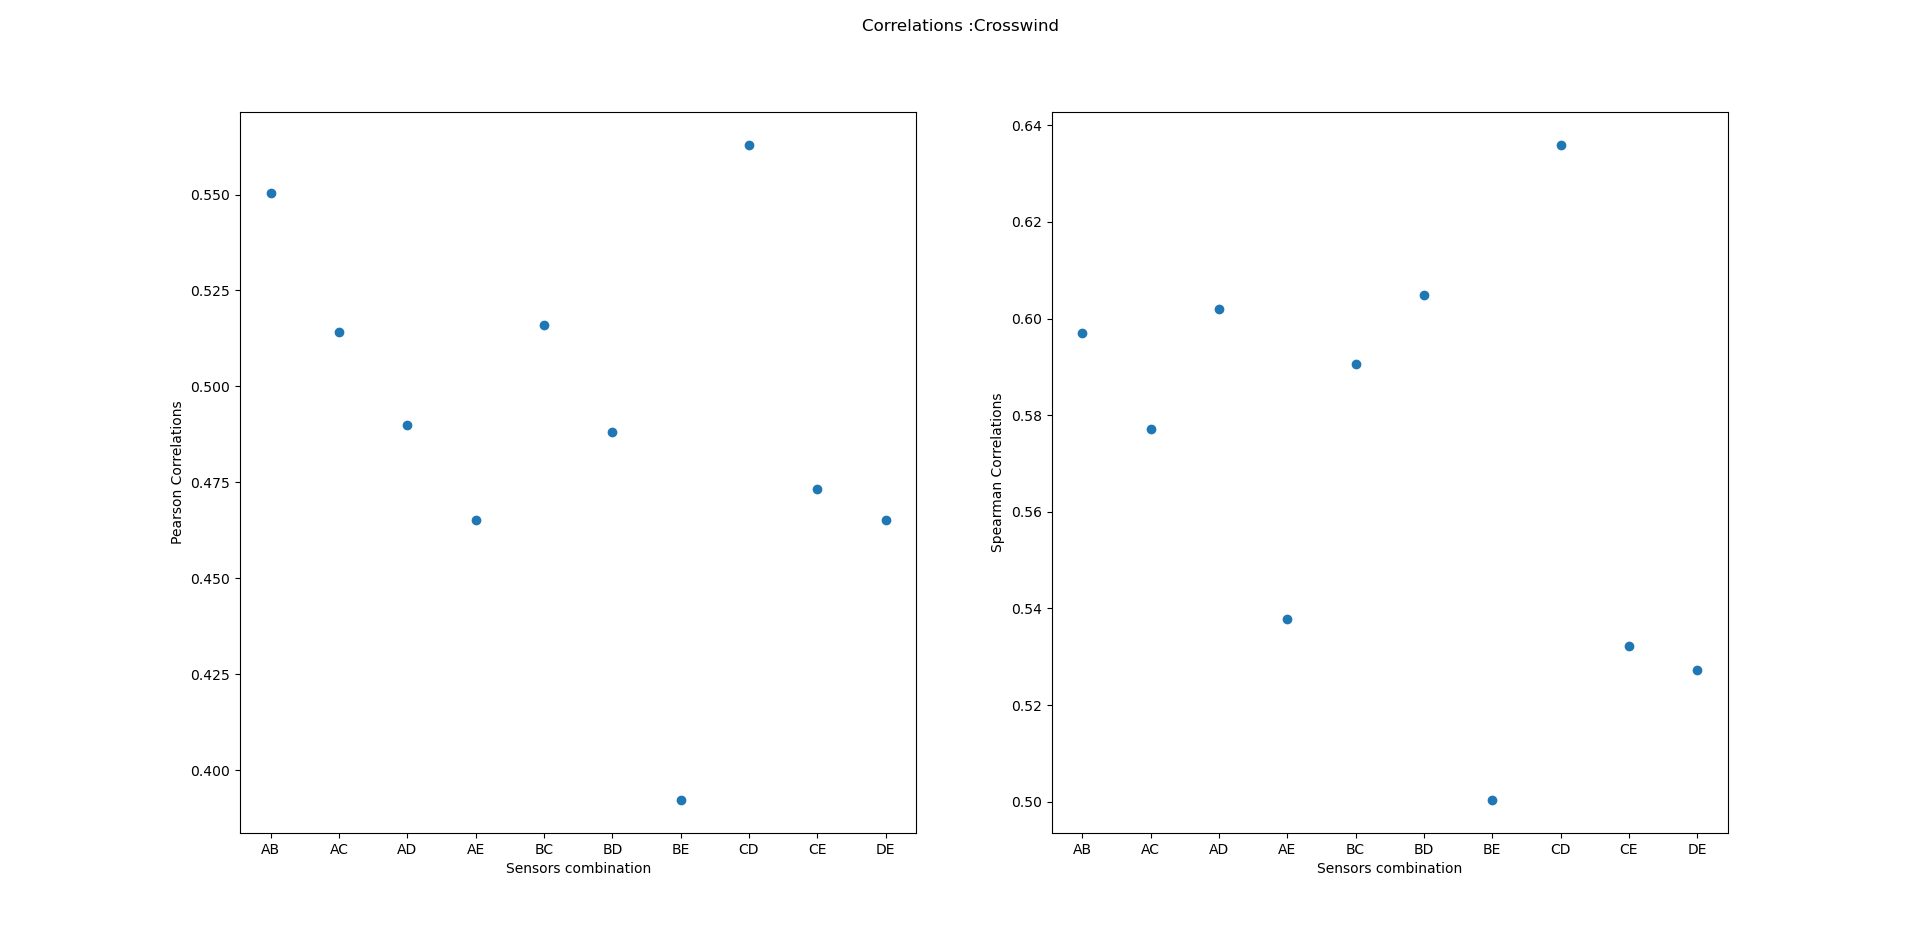
\includegraphics[width=\textwidth]{images/Correlation_Crosswind_Speed.png}
                \caption{Pearson’s and Spearman’s rank coefficients: Crosswind Speed}
                \label{fig:Correlations}
            \end{figure}

            \begin{table}[H]
            \centering
            \scalebox{0.5}{
                \begin{tabular}{lcccccc}
                \textbf{Sensors} & \textbf{\begin{tabular}[c]{@{}c@{}}Pearson's Rank Coefficients\\ Temperature\end{tabular}} & \textbf{\begin{tabular}[c]{@{}c@{}}Spearman's Rank Coefficients\\ Temperature\end{tabular}} & \textbf{\begin{tabular}[c]{@{}c@{}}Pearson's Rank Coefficients\\ Wet Bulb Globe\end{tabular}} & \textbf{\begin{tabular}[c]{@{}c@{}}Spearman's Rank Coefficients\\ Wet Bulb Globe\end{tabular}} & \textbf{\begin{tabular}[c]{@{}c@{}}Pearson's Rank Coefficients\\ Crosswind Speed\end{tabular}} & \textbf{\begin{tabular}[c]{@{}c@{}}Spearman's Rank Coefficients\\ Crosswind Speed\end{tabular}} \\
                AB               & 0.9880961160961126                                                                         & 0.9873789546525072                                                                          & 0.9912595533881619                                                                            & 0.9921324359540058                                                                             & 0.5503525849570334                                                                             & 0.5969825624049757                                                                              \\
                AC               & 0.9886087185252328                                                                         & 0.9882920066209426                                                                          & 0.9918958502071857                                                                            & 0.9924720182971508                                                                             & 0.5140508798931707                                                                             & 0.5772288910798762                                                                              \\
                AD               & 0.985613462024903                                                                          & 0.9846272388693882                                                                          & 0.9870139489166734                                                                            & 0.9882919234478525                                                                             & 0.4898950130186947                                                                             & 0.6018890586328168                                                                              \\
                AE               & 0.9692047916162694                                                                         & 0.9717698000821421                                                                          & 0.9498286924654165                                                                            & 0.9491275351688659                                                                             & 0.4651246851197132                                                                             & 0.5378446650454964                                                                              \\
                BC               & 0.9844851698356611                                                                         & 0.9854401094930247                                                                          & 0.989729693523277                                                                             & 0.9898635757569907                                                                             & 0.5161024168073268                                                                             & 0.5906839137964633                                                                              \\
                BD               & 0.9862654029844026                                                                         & 0.9860487230587479                                                                          & 0.9878642090483689                                                                            & 0.9873748114350143                                                                             & 0.48802933817375793                                                                            & 0.604818772469813                                                                               \\
                BE               & 0.9720897382360566                                                                         & 0.976859613455202                                                                           & 0.9544089298174472                                                                            & 0.9569004735371843                                                                             & 0.39214871017571246                                                                            & 0.500281381925235                                                                               \\
                CD               & 0.9887428724207228                                                                         & 0.9881855891390963                                                                          & 0.9918205586342298                                                                            & 0.9914219338897717                                                                             & 0.5628881993613148                                                                             & 0.6359061682587346                                                                              \\
                CE               & 0.9720972146615451                                                                         & 0.9773424118180742                                                                          & 0.9492695317424182                                                                            & 0.9493455874960454                                                                             & 0.47323322832012416                                                                            & 0.5322320929791761                                                                              \\
                DE               & 1, 0.9713657061948087                                                                      & 0.9758482550943606                                                                          & 0.9480902122116064                                                                            & 0.9487020195244296                                                                             & 0.46519207768485027                                                                            & 0.5273253265612854                                                                             
                \end{tabular}
            }    
            \end{table}
            
            Considering the three (3) scatter plots and taking into account the results from all the above diagrams (histograms, boxplot) we can estimate sensors’s possible position. It is noted that since the differences between the coefficients are almost fractional there is more than one possible positions for sensors A, B, C and D, since for sensor E all the data we have leads to the initial assumption that is located in a remote place.
            
            The following Figure (24) shows the possible sensors's position.
            \begin{figure}[H]
            \centering
                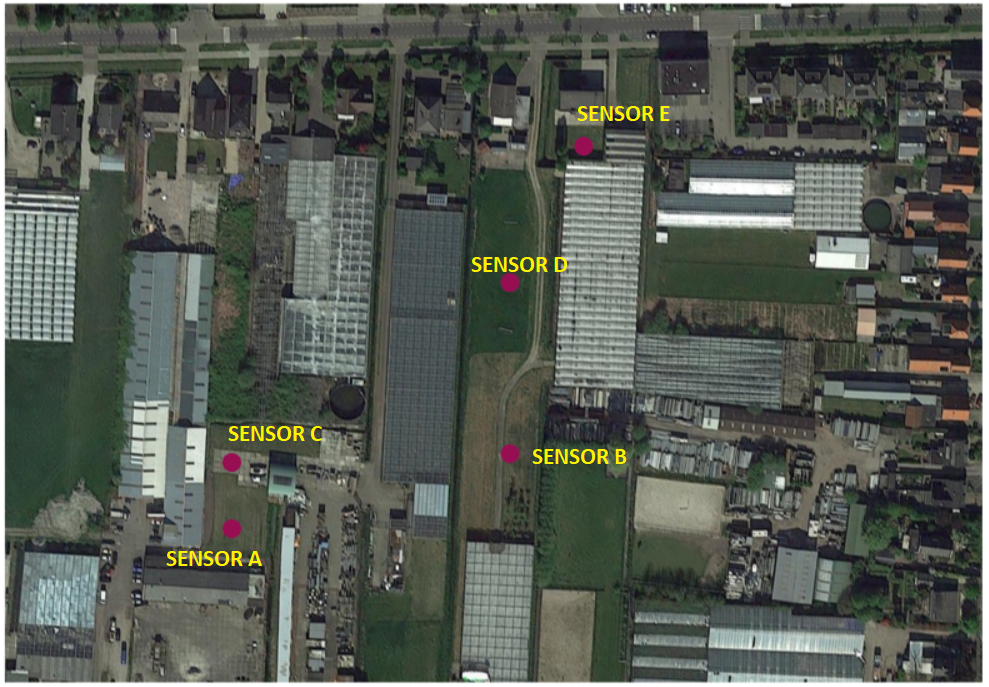
\includegraphics[width=\textwidth]{images/sensors.PNG}
                \caption{Sensors possible location}
                \label{fig:Possible Location}
            \end{figure}
           
\section{Part IV}

        \subsection{Q.1: Plot the CDF for all the sensors and for variables Temperature and Wind Speed, then compute the 95/100 confidence intervals for variables Temperature and Wind Speed for all the sensors and save them in a table (txt or csv form).}
        \begin{figure}[H]
        \centering
            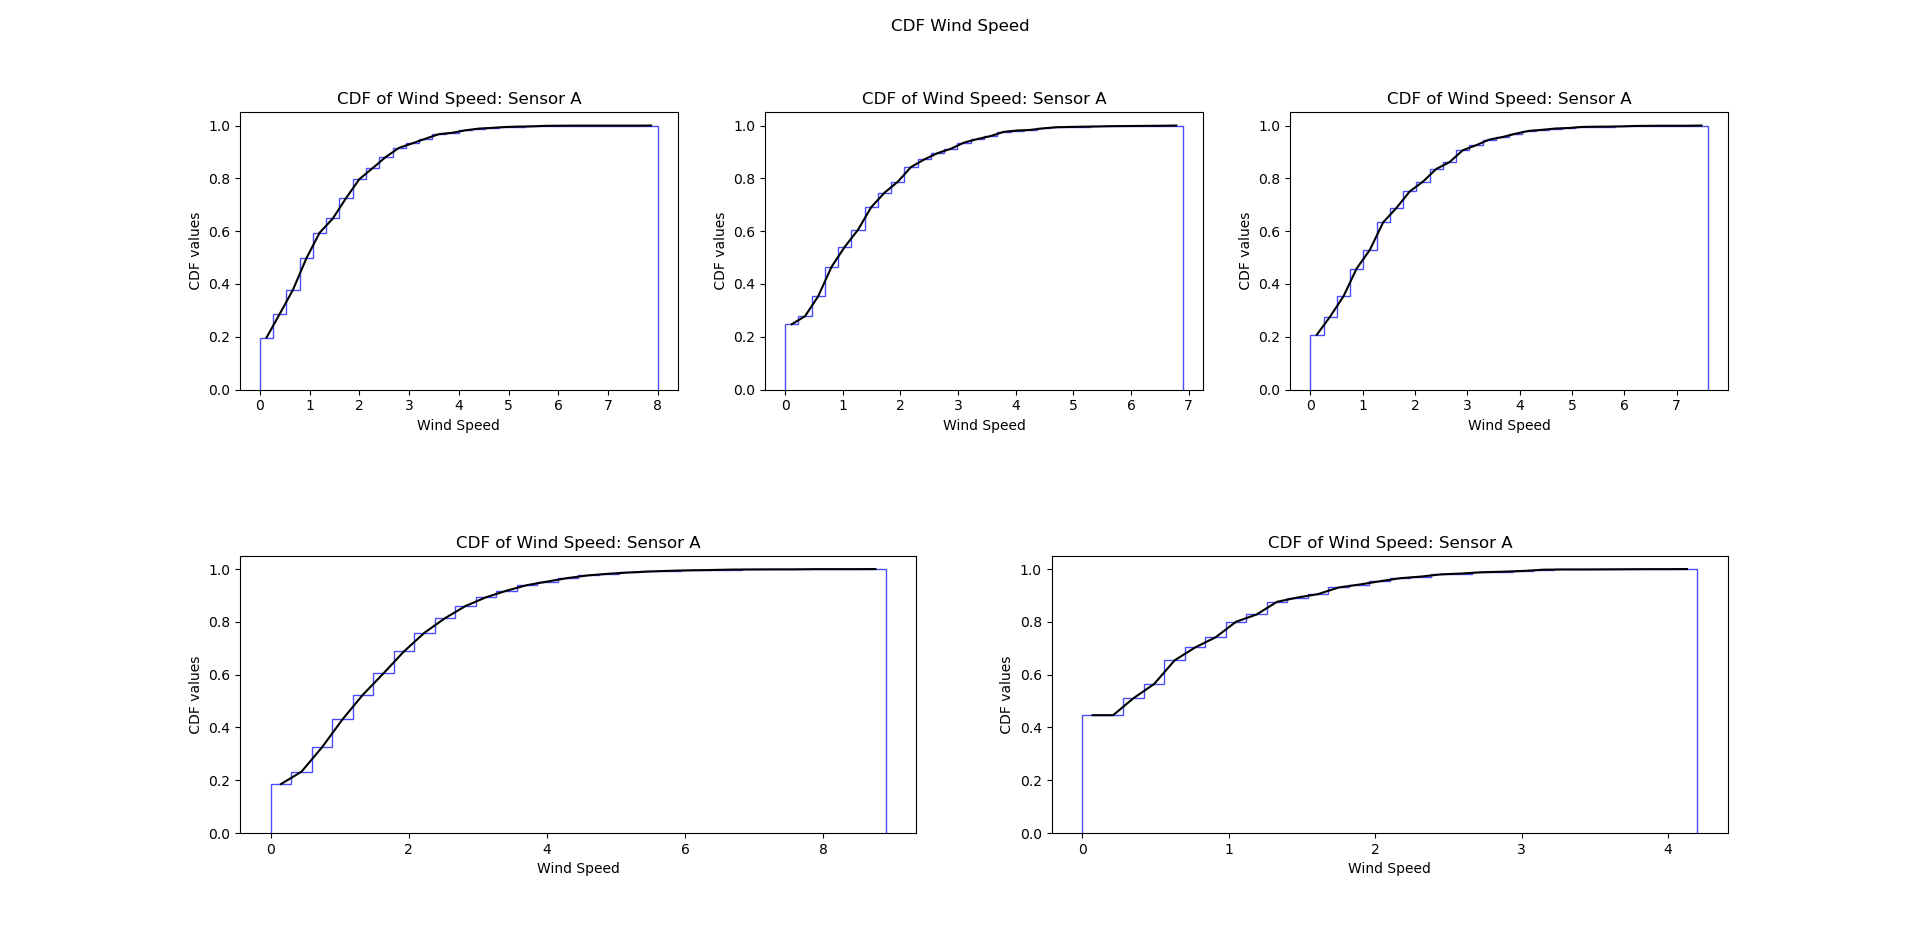
\includegraphics[width=\textwidth]{images/CDF_Wind_Speed_5_sensors.png}
            \caption{Cumulative Density Function for Wind Speed}
            \label{fig:CDF}
        \end{figure}
        
        \begin{figure}[H]
        \centering
            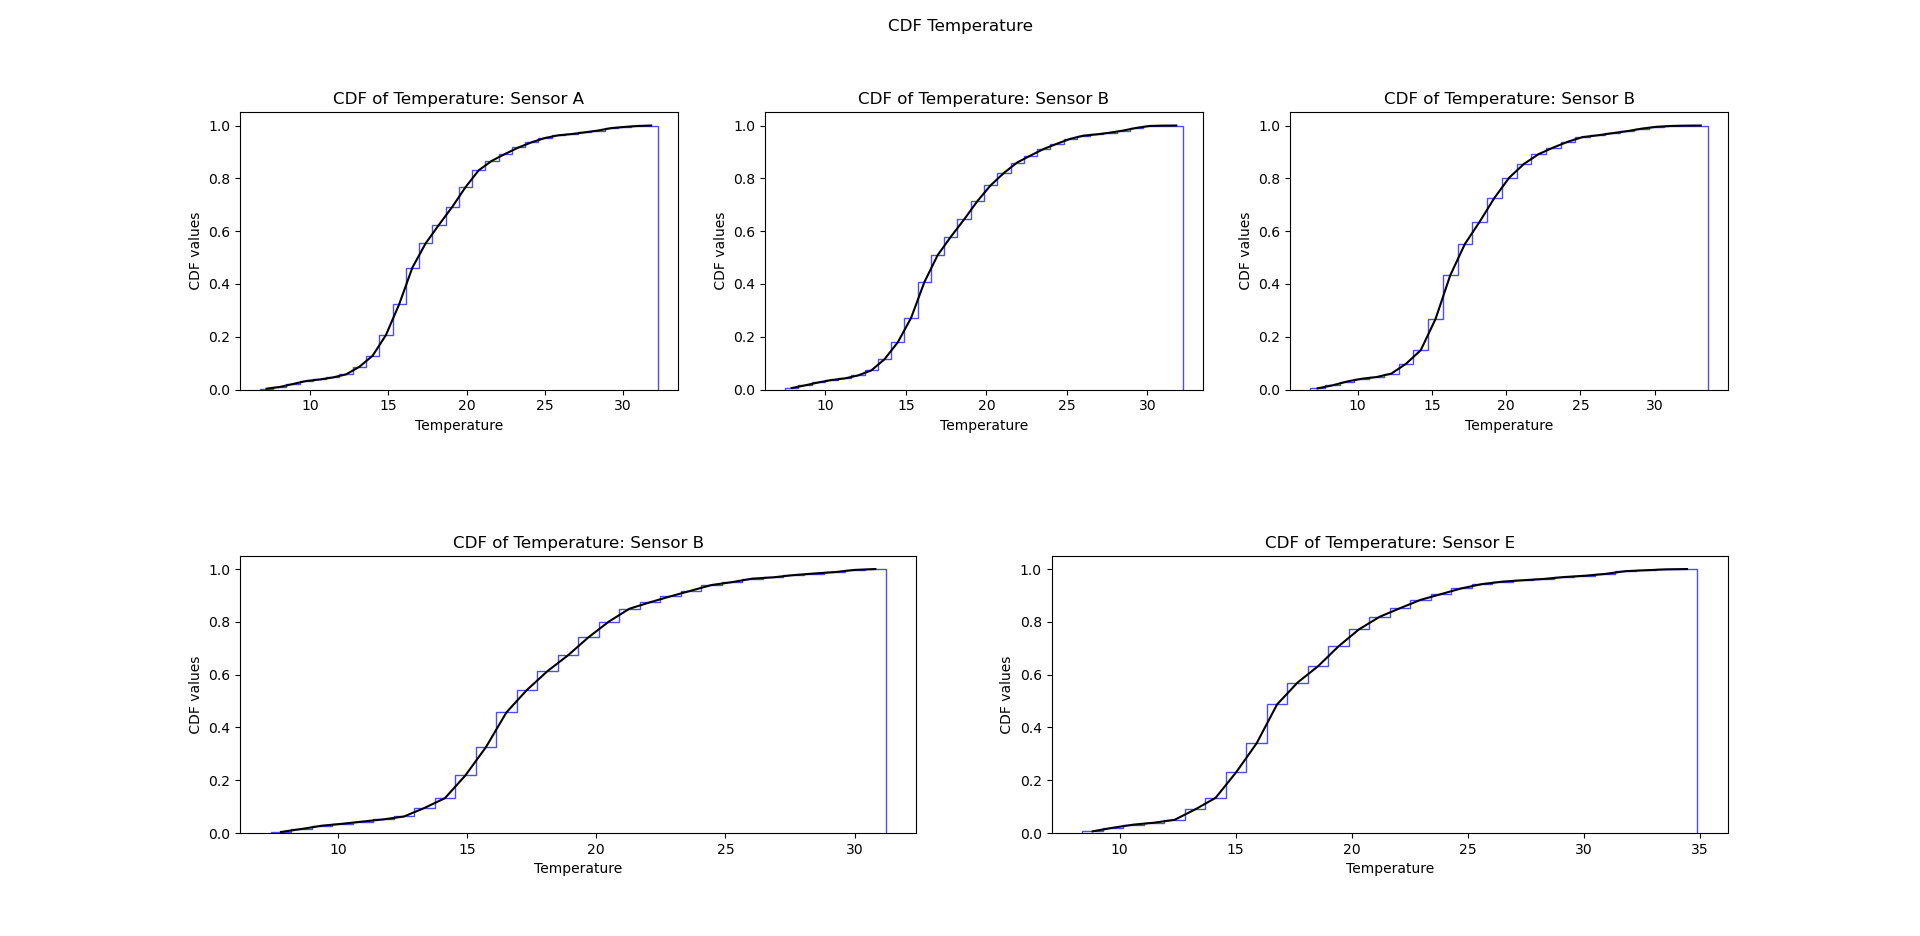
\includegraphics[width=\textwidth]{images/CDF_Temperature_5_sensors.png}
            \caption{Cumulative Density Function for Temperature}
            \label{fig:CDF}
        \end{figure}

            \begin{figure}[H]
            \centering
                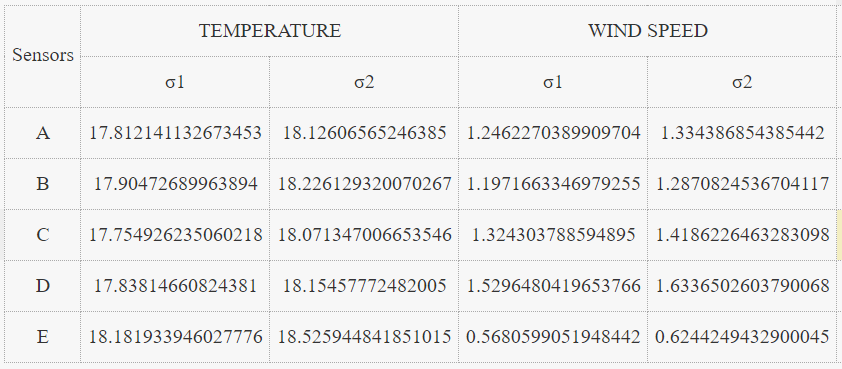
\includegraphics[width=0.5\textwidth]{images/intervals.PNG}
                \caption{95/100 Confidence intervals for Temperature and Wind Speed}
                \label{fig:Confidence intervals}
            \end{figure}

        \subsection{Q.2: Test the hypothesis: the time series for Temperature and Wind Speed are the same for sensors: 1) E, D; 2) D, C; 3) C, B; 4) B, A.
        What could you conclude from the p-values?}
    
            In order to draw conclusions regarding p-values for the variables of Temperature and Wind Speed a null hypothesis should specified. In our case the former hypothesis is “the time series for each variable is the same for all sensors”. That means:
            
            
                    \begin{equation}
                             x_1 - x_2 = 0
                    \end{equation}
                            
            $x_1$: Temperature values for sensor E

            $x_2$: Temperature values for sensor D

            Since the hypothesis test determines that the times series are the same ($x_1$ = $x_2$) it will be used the two-tailed probability. For the test was specified the $\alpha$ level (significance level) to be equal to $\alpha $ = 0.05 (95/100 confidence intervals). The next step is the computation of the probability value. The results are the following:
           
            \begin{figure}[H]
            \centering
                    \begin{subfigure}[b]{0.4\linewidth}
                      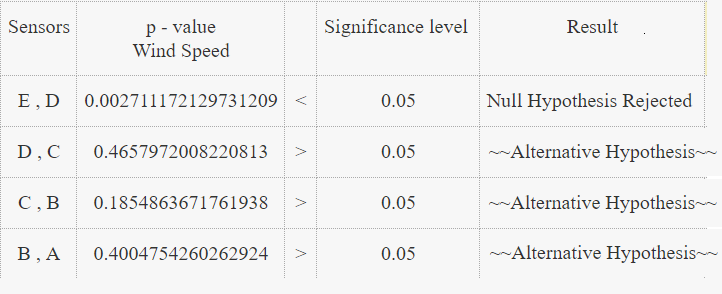
\includegraphics[width=\linewidth]{images/p_value_ws.PNG}
                      \caption{Probability values for Wind Speed measurements}
                    \end{subfigure}
                    \begin{subfigure}[b]{0.4\linewidth}
                      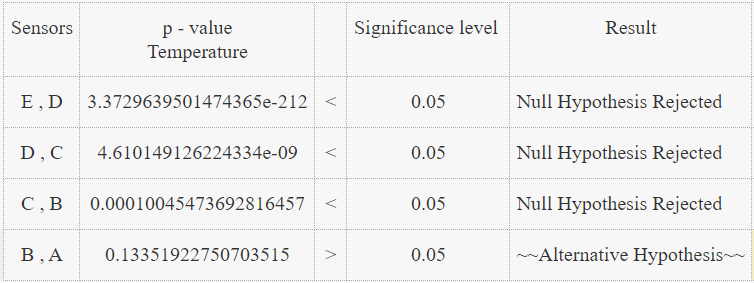
\includegraphics[width=\linewidth]{images/p_value_t.PNG}
                      \caption{Probability values for Temperature measurements}
                    \end{subfigure}
                    \caption{P - values}
                    \label{fig:Histogram}
                \end{figure}

        In order to accept or reject the null hypothesis the above results compared with the $\alpha$ level. If the former value is lower than the latter one the null hypothesis rejected (stastical significant). The lower the probability value, the more confidence you can have that the null hypothesis is false and so there is stronger evidence in favor of the alternative hypothesis \cite{newtest}.The alternative hypothesis states whether the population parameter differs from the value of the population parameter stated in the conjecture. On the other hand, failure to reject the null hypothesis means that you do not have sufficiently strong data to reject it (we cannot conclude that a significant difference exist or we accept directly the opposite).
\section{Bonus question: Your “employer” wants to estimate the day of maximum and minimum potential energy consumption due to air conditioning usage. To hypothesize regarding those days, you are asked to identify the hottest and coolest day of the measurement time series provided. How would you do that? Reason and program the python rutine that would allow you to identify those days.} 

In order to estimate the hottest and coolest day of the given measurement time series there should be followed the next steps:
\begin{itemize}
    \item Data control: focus on date-time-measurements for the Temperature variable
    \item Computation of mean temperatures/day: at this point, the averages of the daily temperatures calculated in order then to identify their maximum and minimum values, for the study period.
\end{itemize}

Since the employer does not determine a certain date / hour frame of calculations (ex. specific hours of the day, morning – night etc.), determining the average temperature per day and then the minimum and maximum values, seems the most logical solution. 

\begin{figure}[H]
\centering
    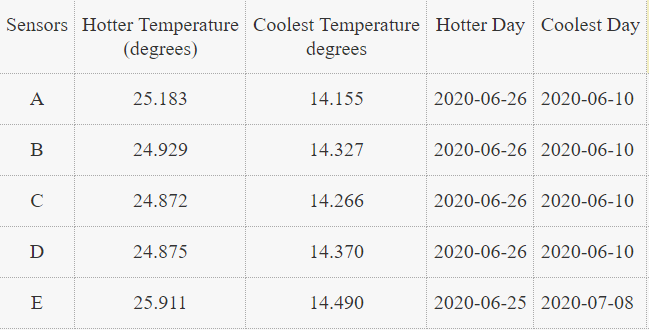
\includegraphics[width=0.5\textwidth]{images/bonus.PNG}
    \caption{Hypothesize the day of maximum and minimum potential energy consumption due to air conditioning usage}
    \label{fig:Confidence intervals}
\end{figure}

From the table above is noticed that the sensors A, B, C and D have a maximum temperature at almost 25°C in 2020-06-26 whilst sensor E has its highest value of temperature one day before (2020-06-25). On the other hand, the lowest temperature that sensors had at the study period was 14°C. Sensors A, B, C and D had that temperature in 2020-06-10 but as far as E sensor is concerned that temperature were reached in 2020-07-08. Regarding these results, we can estimate that the day with the maximum potential energy consumption due to air conditioning usage is 2020-06-25, since that day was the hottest one whilst the day of minimum energy consumption is 2020-07-08 (there is not a high need of air conditioning usage). 
In general when we have the greatest difference between indoor and outdoor temperatures then we have the highest energy consumption due to air conditioning usage. The exact day can be determined when both of the above parameters are known. 

\bibliographystyle{plain}

\bibliography{reference1}

\end{document}